
 %------------------------------------------------------------------------------------------------------------
 % FILE: 			HivmTex.tex
 % AUTHOR:		Ed Johnson
 % DATE:			June, 2005 (starting conversion to LaTeX.
 % PURPOSE:		Final Research Project for Ed Johnson's Masters Degree.
 % PROFESSOR:	Dr. Ljubomir Buturovic
 %------------------------------------------------------------------------------------------------------------
 
 \documentclass[12pt]{report}
 
 \renewcommand{\baselinestretch}{2}
 \usepackage{latexsym}
 %\usepackage{epsf}
 \usepackage{psfig}
 \usepackage{sfsuthesis}
 \usepackage{graphicx}
 
 %Set the bottom margin to 1in
 %\addtolength{\topmargin}{+.5in}
 %\addtolength{\textheight}{.5in}
 
 \tablespagefalse
 \begin{document}
 \title{HIVM - An Application for Prediction of HIV Drug Resistance using Support Vector Machine Algorithms}
 \author{Ed Johnson}
 \submitdate{December, 2006}
\beforepreface
\prefacesection{Abstract}
Drug resistance is a critically important open problem in HIV treatment today.  Current laboratory methods for determining drug resistance have many shortcomings such as high cost, long waits for results, and inability to predict resistance in many circumstances. Our application for predicting drug resistance, hivm, overcomes these obstacles by using a classification algorithm known as Support Vector Machine (SVM). We map HIV amino acid sequences with known drug resistance values to an SVM compatible format that allows us to train a model and then predict drug resistance.   We have conducted a statistical analysis of hivm's ability to predict based on phenotypic datasets. The results show promise for some of the drugs we tested.  However, for the application's true effectiveness to be measured, we would need access to patient response datasets from clinical trials. This data was unavailable for use when implementing this project.
\afterpreface

%----------------------------
%   CHAPTER : INTRODUCTION
%----------------------------

\chapter{Introduction}
\label{cha:Introduction}

Drug resistance is a critically important open problem in HIV treatment today.  A combination drug therapy used on an untreated patient can suppress the virus indefinitely as long as they patient adheres to his drug therapy regimen. However, an individual will have a very large number of HIV strains evolve inside their system within just a few months after infection if left untreated. This happens because the replication mechanism in HIV is very prone to error with more than ten thousand replication errors occurring each day in an untreated individual. As a result of these mutations, there are tens of thousands of HIV+ patients who began their treatment in the 1990s and are now resistant to multiple drugs. This in turn has led to the increased transmission of multi-drug resistant strains of HIV in newly diagnosed patients.\cite{shaferhivinsite}

The long-term goal of the hivm project is prediction of patient response to HIV drug therapy given a genotype of the virus found in the patient. Ultimately, this would lead to a diagnostic test which may aid a physician in prescribing a most efficient HIV drug regimen for a particular patient. 

In order to achieve the goal outlined above, we use machine learning, and in particular a classification algorithm known as 'Support Vector Machine' (SVM). The idea is to train the learning machine (SVM) using known patterns of patient drug resistance for various virus genotypes. The SVM learns the dependency of drug resistance vs. virus genotype with sufficient accuracy as predicted by statistical measures developed during the learning process. Once this is achieved, it can be applied to classifying previously unseen patients (as represented by their viral genotype signatures) into the response/no-response categories.  The hope is that hivm will be able to produce more accurate results, with less computing time and memory than other machine learning applications in this domain.  
\section{Contributions}
\label{sec:Contributions}	

Some of the specific contributions made toward this project are summarized below.

\begin{itemize}

	\item We performed biological,  medical and computer science research needed to determine:
	\item Feasibility of comparing to existing software
	\item New ideas to test in next version of hivm
	\item Software Architecture to support testing of additional ideas.

	\item We implemented a cross-platform, software application in C/C++ to evaluate the performance of support vector machines in this domain. It can run on a commodity computer running 32-bit versions of Windows, Linux, Unix or Mac OSX. 
\newline
	\item We created a suite of unit tests with full regression testing capabilities to aid further development. 

	\item We discovered a problem using the native libsvm\cite{libsvm} where it was generating overly optimistic results. Resolved by creating my own cross-validation mechanism to ensure statistically correct results.

	\item We found and fixed a memory leak in Libsvm. \cite{libsvm_acknowledgments}

	\item We also setup source control servers using CVS and Subversion.
\end{itemize}

The next sections will provide the medical and biological background necessary to understand the project. Following that we will focus on the support vector machine algorithm's mathematics. Then we will discuss implementation of the software, including obstacles and trade offs. This will be followed by results and analysis, conclusion and ideas for further work on this project.


%----------------------------
%   CHAPTER : Biology and Medical Background
%----------------------------

\chapter{HIV Drug Resistance: Biology, Diagnostics, and The Role of hivm}
\label{cha:HIV Drug Resistance: Biology, Diagnostics, and The Role of hivm}
Now, we will review some important biological concepts that are necessary to understand the problem that hivm attempts to solve. 
		
\section{Definition of drug resistance}
\label{sec:Definition of drug resistance}		

As noted by Horn in ``A No-Nonsense Guide to HIV Drug Resistance Testing''\cite{nononsenseguide},
\begin{quotation}
	HIV drug resistance refers to a reduction in the ability of a particular drug or combination of drugs to block reproduction or ``replication'' of HIV. For people infected with the virus, drug resistance can render drugs less effective or even completely ineffective, thus significantly reducing treatment options. Resistance typically occurs as a result of changes-called mutations-in HIV's genetic structure (RNA). Mutations of RNA lead to alterations in certain proteins, most commonly enzymes, that regulate the production of infectious virus. Mutations are especially common in HIV, as this virus reproduces at an extraordinary rate and does not contain the proteins needed to correct mistakes made during copying of the genetic material. HIV relies on many enzymes-such as reverse transcriptase, integrase, and protease-to replicate inside a human cell.  If a mutation of a single site in the reverse transcriptase gene occurs, the change will remain with the virus as long as it replicates or until another copying error alters its form yet again. Some mutations cause the virus to become so weak that it cannot replicate effectively; other mutations may cause the virus to become even more virulent.
	Antiretroviral drugs, generally speaking, disrupt the HIV enzyme's ability for genetic copying, or making virus that can infect other cells. In a person who takes antiretroviral drugs, most of the HIV are killed or prevented from multiplying further. As a result of random mutations that occur on a daily basis, however, some strains of HIV are naturally resistant to the presence of such drugs. That is why treatment with monotherapy (a single antiretroviral drug) is destined to fail.\cite{nononsenseguide} 
\end{quotation}


\section{Current methods for determining drug resistance}
\label{sec:Current methods for determining drug resistance}		

HIV drug resistance occurs when the virus is able to resist the drugs ability to suppress or limit its reproduction. There are currently two tests used to measure for drug resistance. One kind of test is called a genotypic test, the other is called a 	phenotypic test. Resistance testing is useful for both newly diagnosed patients, as well as patients who have been medicating for years and may have developed resistance to their regimen.\cite{seattletreatmentproj}

\section{Definition of Viral Load}
\label{sec:Definition of Viral Load}

Viral load measures the amount of HIV virus in one milliliter of a patient's blood. The higher the viral load, the faster the HIV disease progresses. The viral load test is a valuable tool to determine if antiviral drugs are controlling the infection. The best tests as of this writing can detect viral loads as low as 5 copies per milliliter, though the original tests bottomed out at 10,000 copies per milliliter. Only 2\% of HIV in a patient's body resides in the blood, so viral load tests cannot determine whether a patient has removed all HIV from their body.  US treatment guidelines suggest that anyone with a viral load over 100,000 should be offered antiviral treatment.\cite{aidsorg}

\section{Definition of Genotypic Test}
\label{sec:Definition of Genotypic Test}

As defined by the Seattle Treatment Project,\cite{seattletreatmentproj}
\begin{quotation}
	A genotypic test is a test that examines a specific person's HIV to see if the virus has mutations, and to determine where in the genetic structure of the virus those mutations occur. (Hence the name ``genotypic''.) Any mutations that are identified through this test are then compared with known drug resistant mutation points for all of the currently available HIV drugs. If there is a match between an identified mutation in the specific person's HIV and known drug-resistant mutation points, the virus is believed to be resistant to those drugs where there is a match.
	

	Genotypic testing can be done in people with a viral load under 1,000 because genotypic testing only involves comparing a person's specific HIV mutations to known drug resistant mutation points. The test can be highly predictive of drug resistance for the ``nucleoside analog'' class of drugs (AZT, 3TC, DDI, etc.) and ``non-nucleoside reverse transcriptase inhibitors'' (Sustiva, Viramune, etc.) because these classes of drugs have fairly consistent mutation patterns. However, this test is less predictive of resistance patterns for ``protease inhibitors'' (Crixivan, Fortovase, etc.) since this class of drugs is not always consistent in the pattern of mutations it produces.
	
	Genotypic testing is less expensive and much faster than phenotypic testing. [see next section] Cost ranges from \$300 to \$500 per test, and results are usually available within a week. � The data reported back can be very difficult to understand, even for physicians, so those unfamiliar with how to interpret the test may need to consult with a specialist in HIV care who is familiar with how to read and interpret the results. \cite{seattletreatmentproj}
\end{quotation}

\section{Definition of Phenotypic Test}
\label{sec:Definition of Phenotypic Test}

As defined by the Seattle Treatment Project,\cite{seattletreatmentproj}
\begin{quotation}
	In a phenotypic test, a person's blood is divided into many test tubes. A different HIV drug is mixed into each test tube. The virus in each tube is then watched to see which drugs it is able to rapidly produce in the presence of. The amount of drug in each test tube is then increased until it is enough to stop virus reproduction. Based on the amount of drug necessary to stop viral reproduction, a resistance ``profile'' is created. A simplified way to think of the resistance profile for each drug is:
	
	   1. Low-level resistance: when a 2 to 4 fold [2 fold = 200\%] increase in the amount of drug in the test tube is needed to stop HIV reproduction.
	
	   2. Some resistance: when a 4 to 10 fold increase in the amount of drug in the test tube is needed to stop HIV replication.
	
	   3. High-level resistance: when a 10 fold increase or greater in the amount of drug in the test tube is needed to stop HIV replication. 
	
	Drugs which have a ``low-level resistance'' or ``some resistance'' may still work for the individual person as a part of combination therapy. Drugs which have a ``high-level resistance'' profile are believed to be ineffective in suppressing the virus, and increasing the dosage levels is not thought to be effective. Additionally, consuming HIV drugs at can produce severe side effects in patients.
	
	Phenotypic testing is generally most effective when a person's viral load is greater than 1,000. (For this reason, your provider may not do a phenotypic test if you have a viral load less than 1,000.) A downside to this test is that it does not measure how well different drugs work together in combination (and we know that some drugs can both increase or decrease how well other drugs work when used in combination with each other.) Phenotypic testing is very expensive, and costs about \$1,000 each time the test is done. Also, it takes about 4 to 6 weeks to test a specific person's HIV against all the various drugs. As with genotypic testing, the results can be difficult to interpret and your provider may need to consult with an HIV specialist who knows how to read and interpret this test to make specific drug recommendations.\cite{seattletreatmentproj}  
\end{quotation}

\section{hivm's goals for improved drug resistance testing}
\label{sec:hivm's goals for improved drug resistance testing}

Regarding genotypic testing, the current methods are not good for predicting resistance to the Protease Inhibitor class because ``this class of drugs is not always consistent in the pattern of mutations it produces''. \cite{seattletreatmentproj} hivm has been designed for predicting drug resistance of this case.

Regarding phenotypic testing, the current methods are time consuming and expensive. A physician needs to prescribe the first anti-HIV combination before the 4-6 week delay for phenotypic results.  hivm has a much faster and cost effective turnaround. More importantly, hivm is predicting resistance, rather than reacting to existing resistance.  During the first 4-6 weeks, a newly diagnosed HIV patient must start treatment. Due to the high mutation rate of HIV, even four weeks of incorrect therapy could have severely detrimental effects for the patient's long term prognosis. On an individual basis, hivm should be iteratively run and validated against phenotypic testing. Hence, patients should be periodically retested to see if their HIV strains are mutating during treatment. Individualized patient treatment that changes and adapts to the rapidly mutating virus could be far more effective than a static one-time assessment of a patient's HIV condition.

In addition, a mutation may mean that a HIV strain does not reproduce as efficiently as the wild type, even when not in the presence of any anti-HIV drugs.  Normally, this strain would not be able to use the body's resources as well as normal HIV, and would quickly be wiped out. However, if an HIV drug is actively preventing the wildtype from reproducing , then one of the reproductively inferior strains may now have the most access to the body's reproductive facilities. If the current drug does not bind well to the mutant strain because the binding site has changed, then though this strain may not grow as fast as the wildtype, but it will still increase the infection. It will still destroy the patients immune system, but at a slower rate than the wildtype of HIV.

Since HIV strains with similar sequence of amino acids have a similar binding sites for the drug, we may infer a similar binding affinity to a given drug. We use a variation of the  Smith-Waterman algorithm known as Local Alignment to produce a score that computes the similarity of two amino acid sequences.  The function we are studying is the binding affinity of a drug to an HIV enzyme.  We expect the sequence similarity to be the best predictor of function that we have at our disposal.

Combinations of drugs from at least two of the four available drug classes are usually required to achieve durable HIV suppression. Thus HIV cross-resistance to multiple drugs significantly limits treatment options. In other words, if a doctor's first attempt to treat an HIV patient uses drugs that the patient already won't respond to, then the chances of the patient suppressing HIV decrease dramatically. However, if the doctor calculates the correct drug combination the first time, then the patient has a great prospect of suppressing HIV indefinitely and living a healthy normal life.  Though this prescription will be the single most important decision in the patient's treatment, physicians currently have very limited resources available to help them make this decision.

While phenotypic and genotypic tests provide a useful guess as to an HIV strain's resistance to various drugs. The fact is that the human body is a far more complex setting for this reaction to take place, and there are often unexpected results that do not match up directly to the phenotypic and genotypic tests.  Clinical trials are the most useful source of data for drug resistance because they provide inside into true drug resistance behavior in a human body, where it matters.

\section{Limitations in hivm model vs. the real world biology of the problem}
\label{sec:Limitations in hivm model vs. the real world biology of the problem}

First, we are testing with phenotypic and genotypic datasets because we do not yet have access to clinical trial datasets. While hivm can assess whether a drug can stop the growth of HIV in a lab environment, clinical trial patient response results would be the gold standard to see if we can predict resistance in patients.

Secondly, we can only produce prediction models based upon one viral genotype's resistance to one drug at a time. In reality, the factors of drug resistance are much more complex. For instance, every single patient is treated with three at least anti HIV drugs at once, and the three drugs come from three different classes of anti HIV drugs. 

In addition, we do not have data of a given viral genotypes resistance in the presence of more than one drug at a time. It is very, very important to predict how HIV variants will exhibit complex cross resistance to multiple drugs.  ``A major problem with genotypic testing is that it will miss unknown gene mutations. Also, while the effects of some mutations are clear-cut, this is not always true. A mutation that does not cause resistance by itself could lead to resistance when combined with other mutations. Also, resistance to one drug sometimes results in increased sensitivity to another. One example is that resistance to 3TC reduces resistance to AZT.'' \cite{projinfgenopheno}

Patient response results from clinical trials should help us to overcome these limitations because patient's are normally treated using combination therapy. Therefore, we would train hivm on the results of combination therapy, and our training model would contain information about cross resistance and other factors that may not have been quantified in a lab setting.

The principal resource we will use in this project is the Stanford HIV
Drug Resistance Database \cite{hivdb}, developed under the guidance of Prof. Robert Shafer. It contains a rich collection of documentation and data related to the problem we are studying. In particular, the Drug Resistance Notes sections contains crucial scientific background for the problem of HIV drug resistance.

%----------------------------
%   CHAPTER : Support Vector Machines 
%----------------------------

\chapter{Support Vector Machines }
\label{cha:Support Vector Machines }
Our software application uses Machine Learning, specifically a class of statistical algorithms known as Support Vector Machines (SVM) published by Dr. Vladimir Vapnik.\cite{vapniknature} Cristianini and Shawe-Taylor describe SVM's as ``learning systems that use a hypothesis space of linear functions in a high dimensional feature space, trained with a learning algorithm from optimization theory that implements a learning bias derived from statistical learning theory.''\cite{svmintro}

There are many advantages inherent in SVM's. SVM can classify large data sets of several thousand points while making very efficient use computer memory.  They can predict previously unseen data well (generalization) by avoiding overfitting to training data.  They have a fast training time compared to competing learning methods such as neural networks.  In addition, they have already been used successfully in homology detection of proteins. Chaerkassky and Mulier note many advantages of SVM in their book, �Learning from Data�, ``the set of approximating functions used in the support vector machine ensures that complexity is controlled independently of the dimensionality of the feature space.  Hence, SVM can use large (infinite) dimensional feature spaces.''\cite{learningfromdata}  This permits the application to accept very large datasets without increasing computational time linearly as more variables are added. 

Additionally Scholkopf notes in ``Machine Learning with Positive Definite Kernels'',\cite{maxplanck}  
\begin{quotation}
	One of the most appealing features of kernel algorithms is the solid foundation provided by both statistical learning theory and functional analysis. Kernel methods let us interpret (and design) learning algorithms geometrically in feature spaces nonlinearly related to the input space, and combine statistics and geometry in a promising way. Kernels provide an elegant framework for studying three fundamental issues of machine learning.
	
	- \textit{Similarity measures} -the kernel can be viewed as a (nonlinear) similarity measure,
	and should ideally incorporate prior knowledge about the problem at hand
	
	- \textit{Data representation} - as described above, kernels induce representations of the
	data in a linear space
	
	- \textit{Function class} - the kernel implicitly also determines the function class which is used for learning. Support vector machines have been one of the major kernel methods for data classification.\cite{maxplanck} 
\end{quotation}

Cherkassky and Mulier further note that unlike competing statistical methods such as neural networks, ``the SVM approach does not attempt to control model complexity by keeping the number of features small. Instead, with SVM the dimensionality of z-space can be very large (infinite) because the model complexity is controlled independently of dimensionality.  The motivation for using the high-dimensional feature space is that linear decision boundaries constructed in the high-dimensional feature space correspond to the nonlinear decision boundaries in the input space.''\cite{learningfromdata}

\section{Two problems overcome by support vector machine in its design}
\label{sec:Two problems overcome by support vector machine in its design}

Chaerkassky and Mulier state,\cite{learningfromdata} 
\begin{quotation}
	The conceptual problem is how to control the complexity of the set of approximating functions in a high dimensional space in order to provide good generalization ability.  This problem is solved by using penalized linear estimators with a large number of basis functions.  The SVM approach results in a constrained quadratic optimization formulation of the learning problem...The computational problem is how to perform numerical optimization (i.e. solve quadratic optimization problem) in a high  dimensional space.  This problem is solved by taking advantage of the dual kernel representation of linear functions. \cite{learningfromdata}
\end{quotation}

\section{SVM Background Definitions}
\label{sec:SVM Background Definitions}

The following concepts will be used in the next sections. They are defined here for the benefit of the reader.

\textit{Hilbert space}: Hilbert Space is a vector space H with an inner product $\left\langle{f,y}\right\rangle$  such that the norm defined by
$\left|{f}\right|$ = $\sqrt{\left\langle{f,f}\right\rangle}$
turns H into a complete metric space. If the metric defined by the norm is not complete, then H is instead known as an inner product space. \cite{wolfram}
 
\textit{VC dimension}: size of largest subset of X shattered by
H (every dichotomy implemented) \cite{biowulf}

\textit{Structural Risk Minimization}: Minimization of a bound on generalization error.

\section{The four key properties of the SVM algorithm}
\label{sec:The four key properties of the SVM algorithm} 

The core SVM concepts are described by Chaerkassky and Mulier,\cite{learningfromdata}

\begin{quotation}
	1. New implementation of the Structural Risk Minimization  inductive principle. Instead of the usual SRM strategy for minimizing the guaranteed risk by minimizing the empirical risk on each element of a structure, the SVM implementation uses a special structure that keeps the value of the empirical risk fixed for all approximating functions but minimizes the confidence interval (for classification problems)...
	
	2. Input samples mapped onto a very high-dimensional space using a set of nonlinear basis functions defined a priori.  It is common in pattern recognition applications to map the input vectors into a set of new variables (features) which are selected according to a priori assumptions about the learning problem.  Theses features, rather than the original inputs, are then used by the learning algorithm.  This type of feature selection often has the additional goal of controlling complexity for approximation schemes where complexity is dependent on input dimensionality.  Feature selection capitalizes on redundancy in the data in order to reduce the problem's complexity.  This is in sharp contrast to the approach taken in the SVM which puts no restriction on the number of basis functions (features) used to construct a high dimensional mapping of the input variables.  For the support vector machine, complexity is controlled independently of the dimensionality of the feature space (z-space).
	
	3. Linear functions with constraints on complexity used to approximate or discriminate the input samples in the high-dimensional space.  The support vector machine uses linear estimators to perform approximation.  Many other learning approaches, such as neural networks, depend on nonlinear approximations directly in the samples space.  Nonlinear estimators potentially can provide a more compact representation of the approximation functions; however, they suffer from two serious drawbacks: lack of complexity measures and lack of optimization approaches which provide a globally optimal solution.   Accurate estimates for model complexity can be obtained for linear estimators.  Optimization approaches exist that provide the  (global) minimum empirical risk for linear functions.  For these reasons the support vector machine uses linear estimation in the high-dimensional feature space.
	
	4. Duality theory of optimization used to make estimation of model parameters in a high dimensional feature space computationally tractable.  In optimization theory an optimization problem has a dual form if the cost and constraint functions are strictly convex.  Solving the dual problem is equivalent to solving the original (or the primal) problem \cite{straingapplied}. For the SVM, a quadratic optimization problem must be solved to determine the parameters of a linear basis function expansion (i.e., dictionary representation). For high-dimensional feature spaces, the large number of parameters makes this problem intractable.  However, in its dual form this problem is practical to solve, since it scales in size with the number of training samples.  The linear approximating function corresponding to the solution of the dual is given in the kernel representation rather than in the typical basis function representation.  The solution in the kernel representation is written as a weighted sum of the support vectors.  The support vectors are a subset of the training data corresponding to the solution of the learning problem.  The weights have an equivalent representation in the high-dimensional feature space. \cite{learningfromdata}
\end{quotation}

\section{Historical Development of SVM}
\label{sec:Historical Development of SVM} 

Chaerkassky and Mulier expound on the development of Support Vector Machines,\cite{learningfromdata}
\begin{quotation}
	
	The conceptual problem of how to control the complexity of the set of approximating functions in a high dimensional space in order to provide good generalization ability is solved by use of the 
	Optimal Separating Hyperplane.\cite{learningfromdata}
	
	A separating hyperplane is a linear function that is capable of separating the training data without error.  Suppose that the training data consisting of n samples
	 $(\textbf{x}_{1},y_{1}),...,(\textbf{x}_{n},y_{n}), \textbf{x}\in\Re^{d}, y\in\left\{+1,-1\right\}$ can be separated by the hyperplane decision function
	
	\begin{center}
	$D(\textbf{x}) = (\textbf{w}\cdot\textbf{x}) + w_{0}$		
	\end{center}
			
	\begin{flushright}
	(3.1)
	\end{flushright}
	
	with appropriate coefficients $\textbf{w}$ and $w_{0}$.  The assumption about linearly separable data will later be relaxed; however, it allows a clear explanation of the SVM approach.  A separating hyperplane satisfies the constraints that define the separation of the data samples: 
	
	\begin{center}
	$(\textbf{w}\cdot\textbf{x}_{i}) + w_{0} \geq$ +1 if $y_{i}$ = +1
	$(\textbf{w}\cdot\textbf{x}_{i}) + w_{0} \leq$ +1 if $y_{i}$ = -1, i=1,...,n	
	\end{center}
		
	\begin{flushright}
	(9.2)
	\end{flushright}
	
	Suppose that the training data consisting of n samples $(\textbf{x}_{1},y_{1}), �,(\textbf{x}_{n},y_{n}), \textbf{x}\in\Re^{d}, y\in\left\{+1,-1\right\}$ can be separated by the hyperplane decision function 
	\begin{center}
	$D(\textbf{x}) = (\textbf{w}\cdot\textbf{x}) + w_{0}$
	\end{center}
	A separating hyperplane satisfies the constraints that define the separation of the data samples:
	 
	\begin{center}
	$y_{i}[(\textbf{w}\cdot\textbf{x}_{i}) + w_{0}]\geq$1,i = 1,...,n		
	\end{center}
	\begin{flushright}
	(9.3)
	\end{flushright}
	 
	For a given training data set, all possible separating hyperplanes can be represented in this form (3.3).  This is an important observation, since it allows separating hyperplanes to be described directly in terms of the training data.  The formulation of the separating hyperplane allows us to solve the classification problem directly.  It does not require estimation of density as an intermediate step.  
	
	\begin{figure}
		\centering
			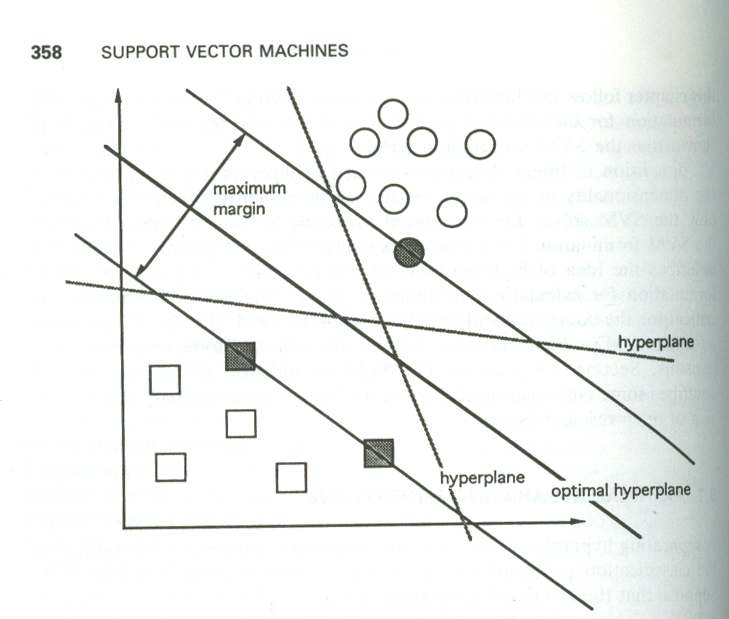
\includegraphics[width=1.00\textwidth]{images/hyperplane1.png}
		\caption{ Separating hyperplanes in a two-dimensional space. An optimal hyperplane is one with a maximal margin. The data points at the margin (indicated in gray) are called the support vectors because they define the optimal hyperplane. \cite{learningfromdata}}
		\label{fig:hyperplane1}
	\end{figure}
	
	The minimal distance from the separating hyperplane to the closest data point is called the margin and will be denoted by $\tau$. A separating hyperplane is called optimal if the margin is the maximum size. It is intuitively clear that a larger margin corresponds to better generalization.  The SVM framework presented below shows how to formally describe an optimal hyperplane and how to determine it from the training data.  The distance between the separating hyperplane and a sample \textbf{x}' is $\left|D(\textbf{x}')\right|/\left\|\textbf{w}\right\|$, as show in the (fig 3.2)  Assuming that a margin $\tau$ exists, all training patterns obey the inequality:
	
	\begin{center}
	$\frac{y_{k}D\left(\textbf{x}_{k}\right)}{\left\|\textbf{w}\right\|}\geq\tau$, k=1,...,n 
	\end{center}
				
	
	\begin{flushright}
	(3.4)
	\end{flushright}
	
	where $y_{k} \in \left\{-1,1\right\}$.	
	
	
	The problem of finding the optimal hyperplane is that of finding the \textbf{w} that maximizes the margin $\tau$.  Note that there are an infinite number of solutions that differ only in scaling of \textbf{w}. To limit solutions, fix the scale on the product of $\tau$ and norm of \textbf{w}, 
	\begin{center}
	$\tau\left\|\textbf{w}\right\|=1$
	\end{center}
	
	\begin{figure}
		\centering
			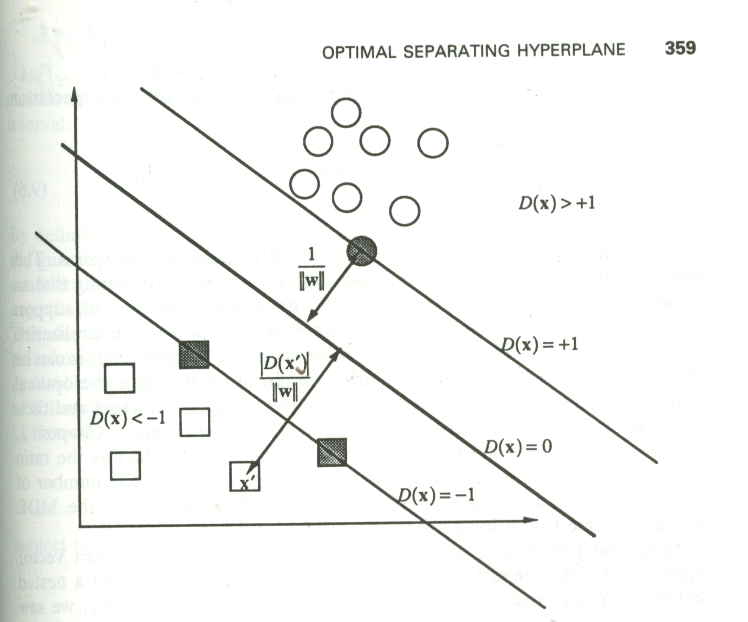
\includegraphics[width=1.00\textwidth]{images/hyperplane2.png}
		\caption{The decision boundary of the optimal hyperplane is defined by points x for which D(\textbf{x})=0. The distance between a hyperplane and any sample \textbf{x}' is  $\left|D\left\langle \textbf{x}'\right\rangle\right| / \left\|\textbf{w}\right\|$.  The distance between a support vector (which defines the margin) and the optimal hyperplane is 1/$\left\|\textbf{w}\right\|$ \cite{learningfromdata}}
		\label{fig:hyperplane2}
	\end{figure}
	
	
	Thus maximizing the margin $\tau$ is equivalent to the minimizing the norm of \textbf{w}.  An optimal separating hyperplane is one that satisfies condition (3.3) above and additionally minimizes
	
	\begin{center}
	$\eta(\textbf{w})=\left\|{\textbf{w}}\right\|^{2}$	
	\end{center}
		\begin{flushright}(3.5)\end{flushright}
	
	with respect to both \textbf{w} and $w_{0}$.  The margin relates directly to the generalization ability of the separating hyperplane.  The larger the margin, the more separation occurs between the classes.  The data points that exist at the margin, or equivalently, the data points for which (3.3) is an equality are called the \textit{support vectors} (fig 3.2). Since the support vectors are data points closest to the decision surface, conceptually they are the samples that are the most difficult to classify and therefore define the location of the decision surface.  It is shown later that the decision surface of the optimal hyperplane is written in terms of the support vectors.
		The generalization ability of the optimal separating hyperplane can be directly related to the number of support vectors.  According to Vapnik \cite{vapniknature} the number of support vectors provides a bound on the expectation of the error rate for a test sample.
	
	\begin{center}
	$E_{n}\left[ Error  rate \right] \leq \frac{E_{n}[ Number of support  vectors ]}{\textit{n}}$
	\end{center}
	 
	\begin{flushright}
	(3.6)
	\end{flushright}
	
	The operator $E_{n}$ denotes expectation over all training sets of size \textit{n}. 
	This  bound is independent of the dimensionality of the space. Assuming 
	that an optimal hyperplane can be constructed with a small number of 
	support vectors (relative to the training set size), it will have good 
	generalization ability \textit{even in high-dimensional space.}
	
	For the hyperplane functions (3.3) satisfying the constraint ${\left\|\textbf{w}\right\|}^{2}\leq c$ , the VC-dimension is bounded by 
	\begin{center}
	$\textit{h} \leq min( r^{2} c, d) + 1$			
	\end{center}
	\begin{flushright}
	 (3.7)
	\end{flushright}
	 where r is the radius of the smallest sphere that contains the training input vectors $(\textbf{x}_{1},...,\textbf{x}_{n}.)$
	
		The factor r provides a scale (in terms of the training data) for c. Notice that it is possible to directly control the complexity of the hyperplane (i.e., the VC-dimension) \textit{independent of dimensionality of the sample space}.   With this measure of the VC-dimension, it is now possible to construct a structure on the set of hyperplanes according to increasing complexity by controlling the norm of the weights $\left\|{\textbf{w}}\right\|^{2}$:
		
	\begin{center}
	$S_{k} = \left\{ \left(\textbf{w}\cdot\textbf{x}\right) + w_{0}: \left\|{\textbf{w}}\right\|^{2} \leq c_{k} \right\}, c1<c2<c3... $			(3.8)
	\end{center}
	\cite{learningfromdata}
\end{quotation}
	
\section{High-Dimensional mapping and Inner Product Kernels}
\label{sec:High-Dimensional mapping and Inner Product Kernels} 

 Chaerkassky and Mulier further describe mapping and kernels,\cite{learningfromdata}
\begin{quotation}
	
	In the last section, it was shown that optimal hyperplanes are good approximation functions because their complexity can be carefully controlled independent of dimensionality.  Therefore, they are capable of providing good generalization ability even for high dimensions. It was shown how to pose the optimization problem of finding the optimal hyperplanes in a manner that allows practical solution even for high dimensional input spaces.   However,  hyperplanes were only described as linear functions in the \textbf{x}-space.  Now, we will describe how to efficiently construct high dimensional sets of basis functions and then determine optimal hyperplanes in this space.  This high dimensional space is called the feature space in order to distinguish it from the input space (\textbf{x}-space).  
	Notice that the optimization problems require the calculation of the inner product between vectors in the \textbf{x}-space, and that this is the only operation requiring the \textbf{x}-values of the training data.  If a large set of basis functions is used (i.e., $\textbf{g}_{j}(\textbf{x}), j=1,...,m)$, then solving the optimization problems would require determining inner products in the feature space defined by the basis functions.   In this section, the set of basis functions is first formally defined, and then the procedure used to compute the inner product of the basis functions is described.  The computation of the inner product corresponds to evaluating an inner product kernel.  Finally, the inner product kernels for a number of common types of basis functions are described.  
	
		Let us denote $\textbf{g}_{m}(\textbf{x}), j=1..m$, as a set of nonlinear transformation functions defined a priori.  These functions map the vector x into an m-dimensional feature space.  hyperplanes can then be created in this feature space rather than in the input space.   For example, the functions $g_{j}(x), j=1...m$, could correspond to polynomial terms of the components of \textbf{x} up to a certain order (including integration terms). Linear decision boundaries in the feature space would then map to polynomial decision boundaries in the input space. The decision function (3.1) becomes 
	\begin{center}
	$D(\textbf{x}) =  \sum\limits_{j=1}^{m} w_{j}\textbf{g}_{j}(\textbf{x})$  						(3.9)
	\end{center}
	
	where the number of terms in the summation depends on the dimensionality of the feature space.   In the dual form this decision function is
	\begin{center}
	\[
	D(\textbf{x}) =  \sum\limits_{i=1}^{n} \alpha_{i}y_{i}H(\textbf{x}_{i},\textbf{x})		(3.10)
	\]
	\end{center}
	
	 The \textit{inner product} kernel H is a representation of the basis functions $\textbf{g}_{j}(\textbf{x}), j=1,...,m$.  It differs from the equivalent kernel representation, since it does not incorporate the parameters estimated from the training data. 
	The \textit{equivalent} kernel representation \textit{is determined after} the approximating function is found, while the inner product kernel \textit{is known a priori }and used to form a set of approximating functions.   For a given set of basis functions $\textbf{g}_{j}(\textbf{x})$, the inner product kernel H is determined by the sum
	\begin{center}
	\[
	H(\textbf{x},\textbf{x}^{'}) =  \sum\limits_{j=1}^{m} g_{j}(\textbf{x})g_{j}(\textbf{x}^{'})
	\]
	\end{center}
	\begin{flushright}
	(9.11)
	\end{flushright}
	
	where m may be infinite.
		Notice that in the form (3.11), the evaluation of the inner products between the feature vectors in a high dimensional \textit{feature space} is done indirectly via the evaluation of the kernel H between support vectors in the \textit{input space}.  This solves the technical problem of evaluating inner products in a high dimensional feature space.    The general expression for an inner products in Hilbert space is
	\begin{center}
		\[
		(\textbf{z} \cdot \textbf{z}^{'}) = H(\textbf{x},\textbf{x}^{'})
	\]
	\end{center}
	(3.12)
	
	where the vectors \textbf{z} and \textbf{z}' are the image in the m-dimensional feature space and vectors \textbf{x} and \textbf{x}' are in the input space.  
	 
		The expansion of the inner product (3.11), (3.12) in the dual representation allows the construction of decision functions that are nonlinear in input space. It also makes computationally possible the creation of a very high dimensional feature spaces, since they do not require direct manipulation. Common classes of basis functions used for learning machines correspond to different choices of kernel functions for computing the inner product.  Below are several common classes of multivariate approximating functions and their inner product kernels:
	
	Polynomials of degree q have inner product kernel:
	
	\begin{center}
		\[
		 H(\textbf{x},\textbf{x}^{'}) = \left[ (\textbf{x},\textbf{x}^{'}) + 1 \right]^{q}
	\]
	\end{center}
	\begin{flushright}
	(3.14)
	\end{flushright}
	
	\textbf{Radial basis functions} of form:
	\begin{center}
		\[
		\textbf{f}(x) = \sin(  \sum\limits_{i=1}^{n} \alpha_{i}\exp\left\{ - \frac{\left|\textbf{x}-\textbf{x}_{i}\right|^{2}}{\sigma^{2}}\right\} )
	\]
	\end{center}
	\begin{flushright}
	(3.15)
	\end{flushright}
	
	where $\sigma$ defines the width of the inner product kernel
	\begin{center}
		\[
		 H(\textbf{x},\textbf{x}^{'}) = \exp\left\{ - \frac{\left|\textbf{x}-\textbf{x}_{i}\right|^{2}}{\sigma^{2}}\right\} )
	\]
	\end{center}
	\begin{flushright}
	(3.16)
	\end{flushright}
	
	Note that the number of basis functions, the center parameters, that correspond to the support vectors and the weights in the output layer are all automatically determined via the optimal hyperplane.  All basis functions have the same width parameter which is specified a priori.\cite{learningfromdata}
\end{quotation}

\section{Support Vector Machine for Classification}
\label{sec:Support Vector Machine for Classification} 

Chaerkassky and Mulier elaborate on SVM classification,
\begin{quotation}
	
	The support vector machine for classification is constructed by applying the concepts of the previous two sections.  The inner product kernel is used to define a high dimensional mapping, and an optimal hyperplane is found in this space.  This corresponds to replacing the inner products in the optimization problems of sections 3.5 with the inner product kernels given in Sections 3.6. First, we will present the final optimization problem statement.  
		
	For classification of no separable data, the decision function is given by
	
	\begin{center}
		\[
		D(\textbf{x}) =  \sum\limits_{i=1}^{n} \alpha_{i}^{*}y_{i}H(\textbf{x},\textbf{x}^{'})
	\]
	\end{center}
	\begin{flushright}
	(3.17)
	\end{flushright}
	
	note that we have dropped the zero-order ``threshold'' term, since it can be represented by including a constant basis function (ie., \textbf{g}(\textbf{x}) =1 ) in the feature space.  the parameters $\alpha_{i}^{*}$, i=1...n, is the solution for the following quadratic optimization problem:
	
	Maximize the functional
	
	\begin{center}
		\[
		Q(\alpha) = \sum\limits_{i=1}^{n} \alpha_{i} - \frac{1}{2}\sum\limits_{i,j=1}^{n}\alpha_{i}\alpha_{j} y_{i}y_{j}H(\textbf{x},\textbf{x}^{'})
	\]
	\end{center}
	\begin{flushright}
	(3.18)
	\end{flushright}
	
	
	subject to constraints
	
	\begin{center}
		\[
		\sum\limits_{i=1}^{n} y_{i}\alpha_{i} = 0, 0\leq\alpha_{i}\leq\frac{C}{n}, i = 1,...,n
	\]
	\end{center}
	\begin{flushright}
	(3.19)
	\end{flushright}
	
	given the training data $(\textbf{x}_{i},y_{i})$, i=1...,n, an inner product kernel H, and regularization parameter C. At present, there is no well-developed theory on how best to select C. In the applications published to date, it is set to a large fixed constant. For the separable case, C = $\infty$.
	
	
		In order to apply the SVM to practical problems, one needs to choose the type of kernel function and the value of C. Rigorous selection of these parameters requires an estimate of the complexity (VC-dimension) and the application of the generalization bound.  Using the generalization bound requires selections for the constants in the bound appropriate for the SVM.  However, ``good'' values of these constants are not known for SVM and there is no accurate estimate for VC-dimension. Therefore, in practice, resampling techniques are used to choose the type of kernel and the value of C.
	\cite{learningfromdata}
\end{quotation}
  This technique was used in our implementation to find optimal SVM parameters, and will be discussed in greater detail in the next section. 


\chapter{Modeling HIV Drug Resistance With hivm}
\label{cha:Modeling HIV Drug Resistance With hivm}

Mathematical modeling of patient resistance to anti-HIV drugs holds promise to improve the clinical standard of care. We designed and built hivm with the aim of providing one such model, based on a machine learning algorithm known as SVM. hivm supports building and evaluating the SVM-based models, as well as generating predictions for previously unseen patient samples using the SVM models. To that end, we recognize the following two modes of operation for hivm.

\textbf{In Practice:}

A blood sample is collected from an HIV+ patient. Then the sample is analyzed by a lab which produces a text file with the individual amino acid sequence of the patient's HIV Protease enzyme. This sequence has usually mutated and is different from the original, wild type HIV Protease enzyme sequence.  The goal is to find out if the patient's mutations make him resistant to a particular HIV drug at a certain drug threshold. A drug threshold could be 10, which means that the patient has to take 10 times the normal dosage of the medication in order to stop HIV from reproducing in his body. The patient's sequence, the drug name, and a drug threshold are input into hivm. The sequence is transformed into an svm-compatible format and the svm algorithm classifies this unknown sequence as resistant or susceptible to that HIV drug at that threshold.

\textbf{In Performance Evaluation:}

Using an svm classifier, one needs to cross-validate on one set of data and test on a separate set of data that is previously unknown to the svm machine. Then the results are compared to see if the svm machine predicted the unknown data at levels similar to the cross-validation results. Cross-validation is the statistical practice of taking a single dataset and repeatedly running an experiment on the data by partitioning it into new, exclusive training and validation groups.\cite{crossvalidation} This gives the user an idea of how well the model will be able to predict on new, unseen data.

The SVM algorithm uses several parameters. In particular, the choices for the penalty parameter, cost, and the width parameter, gamma, make an enormous difference in the performance of the svm algorithm. Therefore, during the model-selection, a grid search is run to find the optimal values for those two parameters. The pair that produce the lowest error rate during cross-validation grid search is chosen and used when classifying the test dataset.

\section{Use Cases}
\label{sec:Use Cases}

Based on the considerations in the Introduction, we identified the following use cases for hivm.

\textbf{Performance Evaluation}\newline
Estimating accuracy of hivm in predicting drug resistance using the viral sequence as input

\textit{model selection}
A user wants to find the most promising training models for use with hivm.
The user provides a single HIVDB formatted dataset file, and hivm will randomly split that file into 2/3 training and 1/3 testing data. If preferred, the user can seed the randomization himself.  Model selection only uses the training dataset. The test dataset is not used at all.\newline

hivm uses the radial basis function kernel as recommended by Hsu, Chang and Line.\cite{libsvmpraticalguide}  The RBF kernel has two important parameters, cost and gamma. The optimal values for these are not known ahead of time, but they are critical in determining the performance of the training model. Therefore, the model selection process performs a search for the optimal cost and gamma parameters using cross validation. The user determines the set of cost, gamma values to test at the command line. For each different parameter pair, hivm runs a 10 fold cross-validation on the training data and saves the performance statistics associated with those parameters to file.

A detailed description of cross-validation used in model selection can be found in the Implementation Challenges section of this document.\newline

\textit{model validation}
A user has run the model selection and seen the resulting ROC curve.
He has chosen a spot on the curve and would like to see how the cost and gamma parameters at that spot fare against the test data. The user gets the same HIVDB dataset as before, and using the same seed, he runs the model validation option for that c,g pair. This provides him with statistics for the parameter pair on the test data. The model validation process will then output the results to file.

\textbf{Prediction for Drug Therapy}

Using hivm to create a drug therapy for a patient

\textit{-model-prediction }(Stub function. Further analysis required before hivm is ready to be used for aiding drug therapy decisions of real patients.)\newline
A user has HIV amino acid sequences from a patient and wants to see hivm's predictions for drug resistance.
For each drug, he feeds in his sequences from a simple FASTA formatted file and receives a single prediction and the probability estimate for the prediction. 

For instance, for drug APV at a dosage threshold 2 times the normal dose, he may receive a prediction that the patient is not-susceptible with a .73 probability that the prediction is correct. The probability estimate has a range of .5 to 1.

\section{Design Decisions}
\label{sec:Design Decisions}

\subsection{Datasets}
\label{sec:Datasets}
As previously stated, clinical trial data was not available when implementing hivm. Additionally, the highest quality dataset came in amino acid sequence format from the Stanford HIVDB website.\cite{hivdbdatasets} The data is provided as a tab delimited text file with each line representing a phenotypic test of a single virus.  We made two trade offs when using this dataset. 

First, we used a less robust dataset in order to test hivm performance. The real test of hivm will be performance on clinical trial datasets. The dataset we used may be easier to predict than clinical trial data, thus giving overly optimistic results.

Secondly, our dataset is composed of amino acids sequences instead of nucleotide sequences. This choice of sequence has made it very difficult to compare hivm performance to that of other prediction software. However, it was the highest quality dataset available when we were implementing hivm.

Additionally, we stopped using the HIVDB dataset for Reverse Transcriptase after spending far too much time trying to clean it up. Though this was an important dataset that represented half of the available drugs to test, we threw it away because it could not be trusted. It has been two years since we told HIVDB the problems with their dataset, and though the readily acknowledge the problems, they have yet to correct them or warn other researchers of their flaws.

\subsection{Issues with RT Dataset}
\label{sec:Issues with RT Dataset}

The individual mutations for isolates do not always match the list of mutations for the same isolate. Since we cannot see the code that creates the dataset, there is no way to know which part is incorrect. The HIVDB team reported that there are errors in the code that generated the datasets, but this code has never been fixed.

Furthermore, the PI and RT datasets have inconsistencies between the two that strongly suggest that they are not created using the same code base. These inconsistencies include different handling of empty strings and mutation lists.

As of September 2006, the datasets are still labeled with the date of November 2004, but in reality they have been changed several times since that date. However, the end user is given no indication of when these releases happened or what errors were fixed in each release. In addition, the dataset formatting is arbitrarily changed between releases. This requires the hivm dataset parser code to be updated and debugged each time, and ruins hivm's backward compatibility with the previous datasets.

Finally, Soo-Yon Rhee, a member of the HIVDB team, stated in June 2006, that they were fixing mistakes in the database as they found them during a two year genotype-phenotype correlation project. However, they would not otherwise review issues with the downloadable datasets used by hivm until this correlation project was completed.

\subsection{CrossValidation}
\label{sec:CrossValidation}
 Leave one out cross-validation refers to partitioning the dataset into groups of size n-1 training data and size 1 validation data. The user repeats this partitioning until each member of the dataset has been tested exactly once. This would be the best type of cross-validation to use, but it proved to be too computationally intensive for our project. Instead we used 10-fold cross-validation which uses 10\% of the dataset for validation in each experiment. After ten experiments, all the data has been in the validation group exactly once.  We felt this method represented a fair trade off of significantly reduced commputation time for marginal degradation in accuracy. 

\subsection{Caching}
\label{sec:Caching}
The model selection process still took far too long to complete. We ran the gnu profiler on the code and found the two functions where 95 percent of the execution took place. Both of these locations were in code that I did not write, so I did not plan to try optimize this code if it could be helped. In fact, we already knew that rewriting portions of the svm library led to the failure of a previous group of students' svm project.  Therefore, we spent the time to create a function to cache the results of the second most computationally intensive function, local alignment, to file. 
Using the cached values can speed up a single parameter pair cross-validation operation on our test server from 25 minutes to about 10 seconds. We test approximately 4225 different cost, gamma pairs for each drug. 

\subsection{Parameter Grid Search}
\label{sec:Parameter Grid Search}
Since we reduced computation by using the 10-fold cross-validation and introduced the cache, we were able to devote more processing time to the parameter grid search. we increased the boundaries of the grid search and made it finer grained than before. This provided more confidence that we selected the optimal cost and gamma parameters for testing each drug.


\subsection{Altering from Traditional Train and Test}
\label{sec:Altering from Traditional Train and Test}
In a typical, trivial svm example, a user would train a model and save that model to file. Then they would use that model file for all future predictions. Our project is more complicated than the trivial example.  At the expense of familiarity with the typical libsvm use, we did work to make hivm more user friendly. hivm was designed to work only with the HIVDB formatted dataset. A typical user would have to go to considerable effort to convert their data to that format, so we can assume that a new user will only be using our HIVDB file. Therefore, we automatically parse and randomly split the HIVDB susceptibility file into training and testing sets. This is far more efficient than splitting by hand, and has the advantage that we can check for data variability by scripting new randomization seeds from the command line.  

Additionally, we never save the libsvm model file as in the trivial example because the svm model cannot be used again as a cache. We must convert data from amino acid sequences into a svm compatible format using local alignment, so the only cache that makes sense is the cache of local alignment values.

We did provide functionality for advanced users who have created their HIVDB dataset(s), so that new and experience users should be accommodated.

\section{Comparison to Similar Software}
\label{sec:Comparison to Similar Software}
In order to publish a paper about hivm, it needs to be compared against another software based method of drug resistance prediction. Unfortunately, the standard  input type for most software is nucleotide sequences, while the dataset for hivm was made from amino acid sequences. The function to transform  nucleotide sequence to amino acid sequence is not one to one and therefore cannot be reversed. Requests to the Stanford HIVDB team for a nucleotide version of their susceptibility datasets have gone unanswered. Details of my research into this area are located in the Further Work Section of this document.



%----------------------------
%   CHAPTER : Implementation
%----------------------------

\chapter{Implementation}
\label{cha:Implementation}

\section{Introduction}
\label{sec:Local Alignment}

We have designed and produced a cross platform C/C++ command line implementation of hivm that is suitable for standalone use or could be integrated into a larger application with some modification. In addition, we have placed hivm under the MIT License\cite{mitlicense} to make it free for both commercial and non-commercial use. 

In this section, we will discuss some of the implementation issues and challenges we faced such as preprocessing of input data, model selection, cross-validation difficulties, and issues debugging a scientific application. In addition, we will outline details of the application itself such as the usage, file structure and software architecture.

\section{Converting Sequence Data into SVM Compatible Format}
\label{sec:Converting Sequence Data into SVM Compatible Format}

SVM requires that each data instance is represented as a vector of real numbers of equal length.\cite{libsvmpraticalguide} Our dataset is in the form of amino acid sequences of different lengths. Hence, we had to solve two problems in order to convert the data to a proper SVM format of equally sized, numerical vectors.

In order to convert our data to numerical form, we chose to compute the sequence similarity among the amino acid sequences. One of the best methods for determining sequence similarity involves computing the ``local alignment score'' of two sequences.  This is based on the Smith-Waterman algorithm \cite{jmolbiol81}, and it is the method used in hivm. Ljubomir Buturovic wrote the code to compute the local alignment scores needed by hivm.

In order to solve the mismatched vector lengths problem, we used a technique known as Empirical Kernel Mapping.\cite{empiricalmap} It involves taking a group of \textit{n} sequences and comparing each sequence to every other sequence in the group. We used local alignment for the comparison function.  This produces an n x n matrix of local alignment scores where each vector is now the same length. This took care of the main problems of preprocessing the sequences for use by the SVM. 

\subsection{HIV Drug Action and Nature of Resistance}
\label{sec:HIV Drug Action and Nature of Resistance}
An amino acid sequence provides the blueprint for a protein. As the resulting protein is created, it folds into a particular three dimensional structure in a process known as folding. This structure determines the functionality of the protein that was based on the amino acid sequence.  In the case of hivm, we are studying two well understood strings of amino acids on HIV. These strings encode two particular enzymes that are
essential to the reproductive cycle of HIV, Reverse Transcriptase and Protease.

These enzymes normally bind with particular molecules in the human body in order to reproduce more HIV. The goal of most HIV anti-viral drugs is to have the drug molecules bind to these HIV enzymes instead of the molecules that HIV would normally bind to.  The drug molecules bind to the  active site of the enzymes, and as long as they are attached to the active site, the cycle of HIV reproduction has been broken.

The most frequently found strain of HIV was used to create modern anti-viral drugs. The drugs are molecules that are known to bind very well to these two active sites. The active sites have a particular three dimensional structure that was determined by the amino acid sequence that encoded them. The drugs also have a site on them that was chosen because it binds very well to one of the two 3D structures at the active sites.

As long as the 3D structure of the active sites remains unchanged, the currently known drugs will do a great job of binding to them and stopping the growth of the HIV infection.  Unfortunately, HIV mutates frequently, and the amino acid sequences for the RT and PI enzymes frequently change.  These mutations are changes in the amino acid sequences that frequently lead to a change in the 3D structure of the active site. This changes the quality of the expected bond between the drugs and HIV enzymes.  Sometimes the drug binds less well to the enzyme, but the enzyme can still bind to the native molecules that it needs for reproduction.  In this case, the HIV infection may have slower growth, but it will still grow. Adding increasing amounts of a particular drug to a patient's system will usually stop the infection, but this increased dosage may cause undesirable and/or toxic side effects in the patient.

Because sequence similarity is usually tightly bound to functional similarity, it is useful to have a method, such as local alignment, to rate similarity between two amino acid sequences. If we know the drug resistance level of a mutated amino acid sequence, then there is a very good chance that a similar amino acid sequence will exhibit the same drug resistance pattern. The drug resistance is determined by the structure of the HIV enzymes' active binding sites, and the structure of the binding sites is primarily determined by the amino acid sequence. 

\section{Libsvm Recommended Procedures for Model Selection}
\label{sec:Libsvm Recommended Procedures for Model Selection}

Libsvm usage is not simple and there are many common pitfalls that new users encounter.  The Libsvm team attempted to rectify this by creating a new users guide. There are many procedures recommended by the creators of Libsvm. \cite{libsvmpraticalguide}

� \textit{Transform data to the format of an SVM software}:\newline
(described above in the Local Alignment section)

� \textit{Conduct simple scaling on the data}:\newline
They note, ``the main advantage is to avoid attributes in greater numeric ranges dominate
those in smaller numeric ranges. Another advantage is to avoid numerical difficulties
during the calculation.''\cite{libsvmpraticalguide}


� \textit{Consider the RBF kernel} $K(x, y) = e^{-\gamma\left\|x-y\right\|^{2}}$:\newline
Lin, Chang and Hsu comment,\cite{libsvmpraticalguide}
\begin{quotation}
	 We suggest that in general RBF is a reasonable first choice. The RBF kernel nonlinearly maps samples into a higher dimensional space, so it, unlike the linear kernel,	can handle the case when the relation between class labels and attributes is nonlinear.
	Furthermore, the linear kernel is a special case of RBF as (Keerthi and Lin 2003)\cite{neuralcomputation}
	shows that the linear kernel with a penalty parameter C has the same performance as
	the RBF kernel with some parameters (C, $\gamma$). In addition, the sigmoid kernel behaves like RBF for certain parameters (Lin and Lin 2003). \cite{linsigmoidkernels}
	The second reason is the number of hyperparameters which influences the complexity
	of model selection. The polynomial kernel has more hyperparameters than
	the RBF kernel. Finally, the RBF kernel has less numerical difficulties. One key point is 0 $<$ $K_{ij}$ $\leq$ 1 in contrast to polynomial kernels of which kernel values may go to infinity ($\gamma$ $x_{i}^{T}x_{j}$ + r $>$ 1) or zero ($\gamma$ $x_{i}^{T}x_{j}$ $+$ r $<$ 1)\cite{libsvmpraticalguide} when the degree is large. Moreover, they note that the sigmoid kernel is not valid (i.e. not the inner product of two vectors) under some parameters.\cite{libsvmpraticalguide} 
\end{quotation}

� \textit{Use cross-validation to find the best parameter C and $\gamma$ }\newline

The RBF kernel has two parameters, C and $\gamma$. The optimal values for these are not known ahead of time, so we must perform a search for the best parameters.  \newline
Lin, Chang and Hsu recommend a simple �grid-search� on C and $\gamma$ using cross-validation. They recommended testing exponentially growing sequences of C and $\gamma$ during the grid search.\cite{libsvmpraticalguide}  

 We searched:
	 $ C = 2^{-16}, 2^{-15}, . . . ,2^{15}, 2^{16} $ and $ \gamma = 2^{-16}, 2^{-15}, . . . ,2^{15}, 2^{6}$


We then used the best penalty parameter C and width parameter gamma to train the whole training set. The cost and gamma that produced the lowest error rate during cross-validation were determined to be the best simple choice.  However, we found a need to use a more advanced analysis of the 'best' cost and gamma parameters that was not described in the Libsvm materials.  We chose a technique known as ROC analysis (Receiver Operating Characteristic).

\section{ROC Analysis}
\label{sec:ROC Analysis}

\subsection{ROC}
\label{sec:ROC}
 According to Dr. William Langdon of the University of Essex,\cite{rocdef}
 
\begin{quotation}The Receiver Operating Characteristics (ROC) of a classifier shows its performance as a trade off between selectivity and sensitivity. Typically a curve of false positive (false alarm) rate versus true positive rate is plotted while a sensitivity or threshold parameter is varied. The curve always goes through two points (0,0 and 1,1). 0,0 is where the classifier finds no positives (detects no alarms). In this case it always gets the negative cases right but it gets all positive cases wrong. The second point is 1,1 where everything is classified as positive. So the classifier gets all positive cases right but it gets all negative cases wrong. (I.e. it raises a false alarm on each negative case).\cite{rocdef}\end{quotation}

A ROC curve allows an HIV expert to choose the trade off points between true positive rate and false positive rate for our SVM machine. In other words, a expert would choose a point on the graph that was best for her situation. That point would give a cost, gamma pair. Then, the expert would train an SVM model with that cost, gamma pair, and predict the classification of her HIV strains using that newly trained model. 

However, for comparing hivm to other software, ROC Curve analysis is not feasible. Commonly used indicators of performance for clinical diagnostic tests such as Sensitivity, Specificity, Error Rate, Diagnostic Odds Ratio and p\_error are more important.

\subsection{Description of hivm ROC Curves}
\label{sec:Description of hivm ROC Curves}
The curves were all generated using the open source plotting utility, gnuplot.\cite{gnuplot} Each point on the ROC curve represents the True Positive Rate (TPR) and False Positive Rate (FPR) of a lg cost, lg
gamma parameter pair used in cross validation during model selection.  As Stuart Baker notes in his paper on ROC, ``By convention, the performance of a classification rule is usually summarized by the following two quantities related to the two types of errors: true-positive rate and false-positive rate.''\cite{baker}

TPR is also known as Sensitivity and FPR is defined as 1 - Specificity.  We will refer to each lg cost and lg gamma data point as a c,g pair for brevity. We produced $65^{2}$ data points in my grid search.  Many c,g pairs produce the
same fpr, but different tpr's, so we pruned the $65^{2}$ data points. First, we sorted all the c,g pairs by fpr in non-descending order. For each fpr, we only kept a c,g pair with the greatest tpr. The ROC curve was completely unreadable without this step because each fpr had multiple tpr's, and it generated a very messy graph. Also, of note, several c,g pairs may produce identical fpr, tpr values. However, only one c,g pair is used in the script.

Now we will describe the relationships among the files that are used to create the ROC curve image. These files are an arbitrary example using drug, ATV, with threshold of 10.

ATV-CrossValb\_t10\_results.csv - contains $65^{2}$ c,g pairs and their full set of statistics. This file is not used to make the ROC curve.

ATV-CrossValb\_t10\_roc\_data\_points.csv - contains only c,g pairs that had the best tpr for each possible fpr. This set is sorted by fpr in non-descending order. This file is used directly by gnuplot to create the image file of the ROC curve.

ATV-CrossValb\_t10\_gnuplot\_script.plt - This the gnuplot script.

Example of a c,g pair as it appears in the gnuplot script:\newline
e.g. set label '' at 0.2,0.25 \# (0,-6)

Breakdown of the c,g pair line:\newline
\begin{itemize}
	\item fpr is .2
	\item tpr is .25
	\item lg c is 0
	\item lg gamma is -6
	\item The label is an empty string. Originally the label was the c,g pair, but
even a modest set of data points makes this illegible.
\end{itemize}

In order to actually pick a c,g pair from the ROC curve, a user must
look at the image and the script. The script's data points are in
non-descending fpr order, so the user must first find a point on the ROC curve with desirable tpr and fpr,
and then scan the gnuplot script down to the point they want. This line in the
script will give them the lg cost, lg gamma that generated the point. With those parameters,
the user will be able to run hivm's unimplemented prediction mode, and they will have an estimated tpr and fpr associated with the output of the prediction. 

In the image, the phrase 'using x:y' refers to the columns from the datafile that are used by the
script. In the included script, it is ``using 4:3'' because the fpr is held in the 4th column, and tpr in the 3rd column of ATV-CrossValb\_t10\_roc\_data\_points.csv. This implementation detail should not be written on the image, but gnuplot writes the plot command on the image by default. 

\begin{figure}
	\centering
		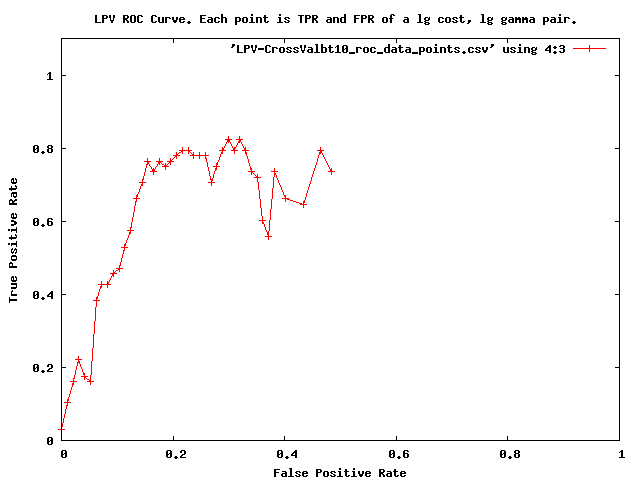
\includegraphics[width=1.00\textwidth]{images/LPV-CrossValbt10_roc_curve.png}
	\caption{The ROC Curve generated by our tests for LPV drug. }
	\label{fig:LPV-CrossValbt10_roc_curve}
\end{figure}


/%\subsection{AUC}
/%\label{sec:AUC}
/%Dr. Tape describes the Area Under a ROC Curve,
/%\begin{quotation}
/%	The area under a ROC curve (AUC) is commonly used as a summary measure of diagnostic accuracy. The accuracy of the test depends on how well the test separates the group being tested into those with and without the disease in question. Accuracy is measured by the area under the ROC curve. An area of 1 represents a perfect test; an area of .5 represents a worthless test.  The area measures discrimination, that is, the ability of the test to correctly classify those with and without the disease. Consider the situation in which patients are already correctly classified into two groups. You randomly pick on from the disease group and one from the no-disease group and do the test on both. The patient with the more abnormal test result should be the one from the disease group. The area under the curve is the percentage of randomly drawn pairs for which this is true (that is, the test correctly classifies the two patients in the random pair). \cite{roc}
/%\end{quotation}


 \section{Implementation Challenges}
\label{sec:Implementation Challenges}

\subsection{Cross-Validation}
\label{sec:Cross-Validation}

First, the total dataset must be partitioned into test and training data. This occurs before we get into the cross validation logic.

\begin{enumerate}
	\item We have a dataset of all possible data.
	\item We randomly split that into 2/3 training data and 1/3 test data. (or  we could
call it learning data and validation data)
	\item We take the 2/3 training or learning dataset and use it to
cross-validate. The 2/3 set is split into learning and validation sets as part of cross-validation. The 1/3 validation set is never used as part of the cross-validation process.  My cross-validation pseudo code in the following section only refers to the 2/3 learning or training dataset.
\end{enumerate}

\begin{verbatim}
           			  Full Dataset
       |                        		    |
2/3 Learning Set            	   	1/3 Validation
       |                                |
Cross-validation function       Validation function
\end{verbatim}

%First, randomly split the full dataset into 2/3 learning dataset and 1/3 validation set.  From this point on, all cross-validation begins with the 2/3 learning dataset. This applies to the libsvm method and our own cross-validation method.

Now, we will discuss the cross-validation in more detail.  Our SVM library was provided by the Libsvm \cite{libsvmpraticalguide} project to perform SVM training, cross-validation, and prediction. The amino acid sequences from the Stanford HIV Database project are of different lengths. Since SVM requires numerical vectors of identical length, we had to perform a pair-wise local alignment comparison of each sequence against all other sequences. In this way, we mapped the original input data into an appropriate feature space for SVM.  Also, because of our special function to map to feature space, we had to write out own cross-validation function.  The Libsvm cross-validation function takes in the 100\% of the data and splits it into folds for you. However, this presupposes that each input vector is independent from the others. In our case, providing one large local alignment matrix would mean that each vector would contain information about every other vector. At that point the libsvm training model would predict a partially known sequence instead of a completely unknown sequence.  In our refactored cross-validation function, we remove all information about the sequence to be predicted from the training model. This ensures that the cross-validation provides honest results. 

we will describe our cross-validation method below.
(To keep it simple, let's say we are dealing with 10 total sequences and 10 fold cross validation.)

%Take a group of sequences from the learning dataset. Compute the pairwise alignment (Local Alignment matrix) of all of them, and feed this matrix into the libsvm cross-validation function. Each vector maps back to a sequence from the original dataset. Each sequence also has a resistance category associated with it. (the simplest case is 0/1. resistant or not). This category threshold(s) is selected by the application's user every time he runs the program.

During one iteration of a 10-fold cross validation, 10\% of the amino acid sequences are randomly selected and logically separated from the remaining 90\% of the amino acid sequences. The 90\% subset is the ``learning set'', and the 10\% subset is the ``validation set''. \cite{vapniknature}

Take all sequences from the learning dataset. Compute the pairwise alignment (Local Alignment matrix) of all of them. Each vector maps back to an amino acid sequence from the learning dataset. Each sequence also has a resistance category associated with it. (the simplest case is 0/1. resistant or not).  The learning set of local alignment vectors and their known category are used to compute an SVM training model. The training model does not contain any local alignment values computed against the sequence of the validation set. 

Our prediction functions worked as follows: Each sequence in the validation set is mapped to feature space by computing it's local alignment value against every sequence that composes the learning set local alignment matrix.  Each validation sequence's identity local alignment value is dropped, which makes the validation sequence's vector of local alignment values the same length as every vector in the learning set. Otherwise, the size of the validation set vectors would each be off by one.

For our validation purposes, we already know the category of each of the validation sequences.  We run the libsvm prediction function on the validation sequences (which we have converted into local alignment vector form). This produces a prediction for the sequence's category. We check to see if this is correct or not and record the value.

As each new cross-validation fold is created from the total set of amino acid sequences, no information about the validation set is ever leaked to the learning set.

Next, we will describe our cross-validation method via a diagram and pseudo-code to further elaborate.

%There is one main difference between a single iteration of the cross validation technique and running a prediction.  In cross validation, the training model contains local alignment value(s) that were created by comparing the model's sequence(s) against the sequence(s) to be predicted. In addition, the sequence to be predicted has it's identity local alignment value in it's vector.


\subsection{Cross-Validation Diagram}
\label{sec:Cross-Validation Diagram}

\begin{verbatim} 
 validation set (VS)                         learning set (LS)
 +--------------------+        +---------------------------------------------+
 |v1|v2|...        |vk|        |l1|l2|l3|              ...                |ln|
 +--------------------+        +---------------------------------------------+

 vi, li are VS and LS viral sequences (i.e., amino-acid strings),
 respectively.

 This is converted into:

 +--------------------+        +---------------------------------------------+
 |x1|x2|...        |xk|        |y1|y2|y3|              ...                |yn|
 +--------------------+        +---------------------------------------------+

 where xi and yi are numeric vectors:

 y1 = [s(l1, l1) s(l1, l2) s(l1, l3) ... s(l1, ln)]
 y2 = [s(l2, l1) s(l2, l2) s(l2, l3) ... s(l2, ln)]
 ..
 yn = [s(ln, l1) s(ln, l2) s(ln, l3) ... s(ln, ln)]
 x1 = [s(v1, l1) s(v1, l2) s(v1, l3) ... s(v1, ln)]
 x2 = [s(v2, l1) s(v2, l2) s(v2, l3) ... s(v2, ln)]
 ..
 xk = [s(vk, l1) s(vk, l2) s(vk, l3) ... s(vk, ln)]

 and s(a, b) is local alignment score between sequences a and b.
\end{verbatim}

\subsection{Cross-Validation Pseudo-Code}
\label{sec:Cross-Validation Pseudo-Code}

for 10 sequential folds
\begin{itemize}
\item createFold:  90\% learning set, 10\% validation set.
\item train on learning set
\item predict on validation set
\item record each fold's results
\end{itemize}

createFold function:
\begin{itemize}
\item Split 100\% of amino acid training data into 90\% amino acid learning set and 10\% amino acid validation set.
\item Convert learning set and validation set of amino acid sequences into SVM compatible vectors
\end{itemize}

SVM compatible vector conversion function:
\begin{itemize}
\item Convert 90\% amino acid learning set of size n to SVM compatible vectors by pairwise comparison. Result is an n x n matrix of local alignment scores. Each row of the matrix represents an amino acid sequence from the learning set.
\item Convert 10\% amino acid validation set of size m to SVM compatible vectors by taking each validation set sequence, and computing its local alignment score with each of the n amino acid sequences from the 				learning set. Result is an m x n matrix of local alignment scores. Each row of the matrix represents an amino acid sequence in the validation set.
\end{itemize}


\subsection{Test Driven Development}
\label{sec:Test Driven Development}
hivm was coded twice. The first time we attempted to use a C++ unit test framework, but the free versions at that time were out of date and very poorly documented.  Over a period of months, we could not find any use group that could explain how to configure their framework for use with my development environment. Making such a framework available from a source code repository for use on different platforms was even more difficult. Fortunately, the test driven development movement has grown rapidly, and when we returned to the project we found that Boost had advanced their C++ framework and documentation considerably.

hivm is a scientific application that attempts to test the performance of a statistical method. No one knows exactly what the final output should be in this case. Therefore, it is impossible to compare the final output from a given set of input data and declare the output correct. While we could not determine that any answer was ever correct, there were several statistical techniques for determining that the answer was very likely wrong.  After several months of programming the first version, we had thousands of lines of code, no unit tests, and an output that we proved was extraordinarily unlikely.  After many fruitless weeks of debugging, we reevaluated the software from a high level. we researched various software development strategies, and decided that the best course of action would be to start over development when we could use a unit test framework. We referred to the old code's architecture and certain implementation details, but the new project started with tests.  Before implementing each new feature, we had to decide how to test it for correctness first. we created a test class for each real class in the project, and began rebuilding hivm. In this way, we were able to create a application built on highly tested individual parts. Then we tested the interfaces of the parts. If we found a error, we wrote a new test to make sure that bug never surfaced again. In this way, we created a much more robust version of hivm.

we found that automated unit testing is a critical component in the development of robust scientific software, particularly in the latter phases of a project. Previously, a new feature request could have unintended consequences in the program and incorrectly change the final output. With regression testing in place, that same feature would break several tests and clearly show the unintended side effects. Ideally, software should never have these ripple effects, but software evolves as it is created and the original architecture can rarely handle all the changes. With the unit tests, we were able to confidently refactor the architecture late in the project.  Additionally, the unit tests helped me track down several bugs and ambiguities in the core support vector machine library that hivm depends on.

One outstanding issue with the Boost C++ unit test frameworks concerns the testing of private class data. While this is easy to do in Java's unit test framework, there was no obvious way to do this with Boost's auto unit tests. We frequently left class data in the public scope during development in order to test the classes. We now route all the unit tests that need access to private members through a special friend class. Tests that use only public interface are kept separate, and this also ensures that my public tests are not 'cheating' by accidentally using knowledge of the internals of the tested class.

\subsection{Boost}
\label{sec:Boost}
Boost is an organization that provides  free, peer-reviewed C++ source libraries that go beyond the functionality included in the C++ Standard Library.\cite{boost} The libraries are used extensively in hivm. They provide many high quality, cross-platform capabilities that the present version of ANSI C++ does not have, and prevent duplication of effort by developers. There was no need constantly reinvent the wheel in C/C++ with Boost available. Additionally, many of the present Boost libraries have been included in the Release Candidate for the upcoming ANSI C++ standard.

Some of the features used in hivm v1 include:
\begin{itemize}
	\item Cross-Platform File system abstraction
	\item Cross-Platform random number generator
	\item Safe Lexical Casting
	\item Tokenizer
\end{itemize}
 
However, the most important library used was  Boost Test. This allowed the setup of the unit tests and regression testing, which were essential to the successful development of the application.

Boost did add some complexity to the software building process because some Boost libraries had to be built for each platform. This was easy to do for 32-bit Windows, but not for Linux variants. So, we created a special build script to build the necessary boost libraries on *nix and Windows platforms in one step. Additionally, the Boost files needed by the script are numerous, which makes downloads from Source Control slower. However, the trade off to save developer effort at the expense of more computer time was acceptable.

Additionally, the Boost license encourages both commercial and non-commercial use.

\subsection{C and Memory}
\label{sec:C and Memory}
The most used programming language in my classes at SFSU was Java. hivm was far more complex than any software in our classes, so managing the memory in an application that uses C and C++ mixed was occasionally very time consuming. Fortunately, in the second implementation of hivm, the Boost unit test framework automatically detects memory leaks in each test. Additionally, we used Visual Leak Detector\cite{leakdetector} and Valgrind\cite{valgrind} to track down more difficult memory leaks, including one in libsvm. Dr. Chin credited me on his website for fixing the memory leak in libsvm. \cite{libsvm_acknowledgments}

\section{Input Data}
\label{sec:Input Data}

The Stanford University HIV Drug Resistance Database group provided the input datasets used for hivm.\newline

HIVDB is provided as a text file with each line representing a phenotypic test of a single virus.  The columns contain information about the virus sensitivity to anti-HIV drugs, and the mutations present in the PI amino-acid sequence of the virus in comparison with the wild-type sequence.

The susceptibility methods in the data set below include only ViroLogic$^{TM}$ test results.  The dataset contains 621 Protease (PI) sequences from 42 references.

Following is a detailed explanation of the columns in HIVDB file.\newline
\textbf{Description of Selected Fields in the DataSet Files}\newline
\textit{Field Name}	Description\newline
\textit{SeqID}	Sequence identifier\newline
\textit{Subtype}	Subtype of sequence\newline
\textit{Method}	Phenotype method\newline
\textit{RefID}	Published reference. View References Table\newline
\textit{Type	Clinical vs. Lab Isolate.} Lab isolates are site directed mutants or results of in vitro passage.\newline
\textit{IsolateName}	Isolate identifier\newline
\textit{Drug Fold	}Fold resistance of Drug X compared to the wild type.\newline
\textit{Drug FoldMatch}	Fold match for Drug X. '=' for most results. '$<$' if result is below the lower limit of the assay. '$>$' if the result is greater than the upper limit of the assay.\newline
\textit{P1...P n}	Amino acid at this position. '-' indicates consensus; '.' indicates no sequence; '\#' indicates an insertion; '~' indicates a deletion and a letter indicates one letter Amino Acid substitution.\newline
\textit{Mutation Lists}	Mutation Lists provided at the far right of the output are lists of mutations present in the sequence. Some lists contain all the mutations, others contain specific sublists.\newline


\section{Example of Sequences from the PI DataSet}
\label{sec:Example of Sequences from the PI DataSet}

The image on the next page shows the highlights of the HIVDB dataset. The figure starts with the identifying information for each phenotypic test. Next, it begins to show the fold resistance of each drug, beginning with APV. For example, the sequence, 2996, required 2.5 times the normal dosage of APV in order to halt replication in the ViroLogic$^{TM}$ test. An '=' symbol in the FoldMatch column means that test results were within normal ranges for the test. Any other symbol means the test result was outside the assay limits, and therefore we discarded those results. Next, we snipped out columns 9 - 53 so that we could show the format of the amino acid substitutions. For example, the column P35 shows that amino acid, D, is substituted for the wildtype amino acid at position 35 in the amino acid sequence of the HIV protease enzyme. This repeats for all 99 amino acids in the sequence. \newline

We snipped out the rest of the substitutions in order to show the Complete Mutation List, Major Mutation List and Minor Mutation list placed at the end of the rows. The mutation lists show amino acid substitutions.

\begin{figure}
	\centering
		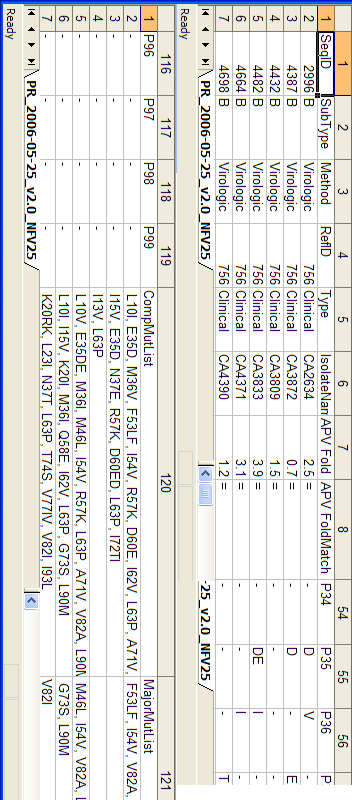
\includegraphics[height=1.00\textwidth]{images/hivdb_dataset.png}
	\caption{Example of HIVDB Protease Inhibitor Dataset. }
	\label{fig:hivdb_dataset.png}
\end{figure}

\newpage

\section{Drugs in the Datasets}
\label{sec:Drugs in the Datasets}


{Protease Inhibitor Drugs}\newline
Amprenavir (APV)\newline
Atazanavir (ATV)\newline
Indinavir (IDV)\newline
Lopinavir (LPV)\newline
Nelfinavir (NFV)\newline
Saquinavir (SQV)\newline
\newline

\newpage

\section{Software Architecture}
\label{sec:Software Architecture}

The software architecture of hivm is detailed in the following sections. Each class is listed along with its  responsibilities. We preferred responsibility driven architecture over data driven architecture as the ability to assign responsibilities to software components strongly influences the robustness, maintainability, and reusability of software components. The architect can assign a responsibility to the ``information expert'', which is the class that has the information necessary to fulfill the responsibility. This helps to attain two of the main goals of a system of classes: high cohesion and low unnecessary coupling. \cite{larman} In addition, focusing on responsibilities also makes it easier to think in the domain of the problem, as it helps maintain an appropriate level of abstraction for each class. In turn, the architect can focus on the interfaces among the classes.

We have included a UML 1.0 chart provides a high level view of the relationships among the classes. The interaction diagram shows the flow of control during a typical execution of hivm.  The UML diagram was created with Microsoft Visio and the State Diagram was created with Borland Togethersoft Community Edition.

\begin{figure}
	\centering
		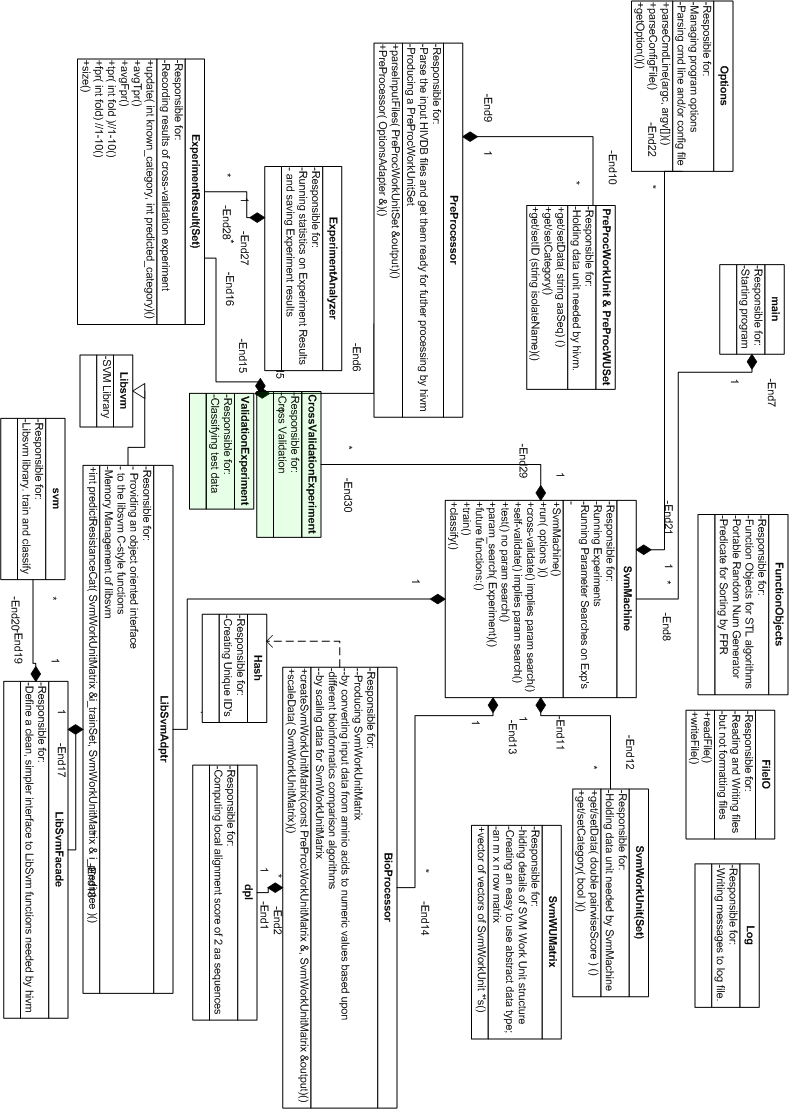
\includegraphics[width=1.00\textwidth]{images/hivm-uml.png}
	\caption{hivm  UML Diagram}
	\label{fig:Hivm_uml}
\end{figure}

\begin{figure}
	\centering
		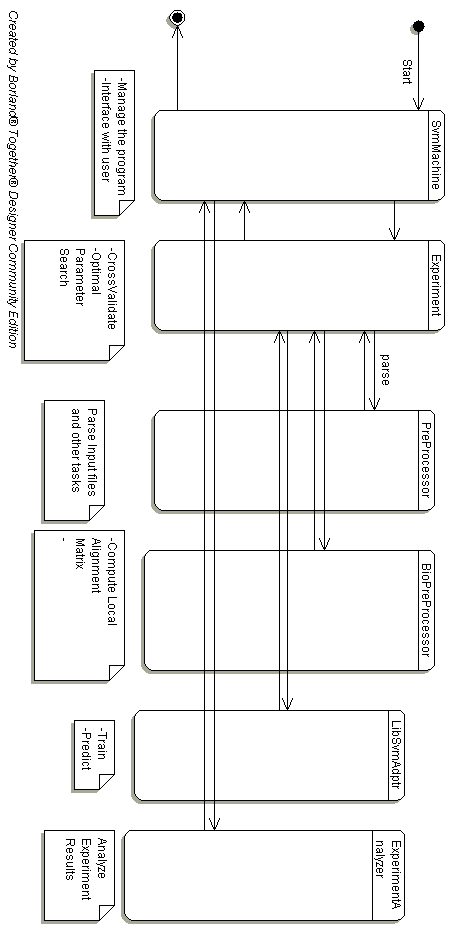
\includegraphics[width=1.00\textwidth, height=1.00\textheight]{images/HivmStateChartv2.png}
	\caption{hivm State Chart}
	\label{fig:HivmStateChart}
\end{figure}

\subsection{Classes}
\label{sec:Classes}

\textit{svm}\newline
LibSVM: Responsible for training and predicting data using support vector machine algorithms

\textit{LibSvmAdapter}\newline
Responsible for providing an object oriented interface between to the libsvm C-style functions, and the rest of hivm. Responsible for memory management and error checking libsvm using full features of C++. 

\textit{LibSvmFacade.hpp}\newline
Responsible for simplifying the interface to the limited set of LibSvm functions needed by hivm

\textit{dpl}\newline
Responsible for producing local alignment scores between two amino acid sequences

\textit{FileIO}\newline
Responsible for reading and writing files 

\textit{Log}\newline
Responsible for writing messages to the log file.
All static functions. Can be used anywhere by any class to make a log entry.

\textit{BioProcessor}\newline
Responsible for converting input data from amino acids to SVM compatible numeric values \cite{jmolbiol81}

\textit{main}\newline
Responsible for starting program

\textit{SvmMachine}\newline
Responsible for running SVM experiments and conducting the SVM parameter search. 

%\textit{DebugHelper}\newline
%Responsible for Static methods to show allow stepping through containers with debugger.

\textit{Hash}\newline
Responsible for creating unique id's

\textit{PreProcessor}\newline
Responsible for parsing the input files and converting them to BioProcessor class compatible format

\textit{Options}\newline
Responsible for parsing the user instructions and options, and then providing that data to the rest of the application

\textit{ExperimentResult}\newline
Responsible for recording results of SVM model selection or model validation experiment.

\textit{ExperimentAnalyzer}\newline
Responsible for calculating and saving statistics from experiment results

\textit{PreProcWorkUnit}\newline
Responsible for holding data generated by the PreProcessor class and used by BioProcessor class

\textit{SvmWorkUnit}\newline
Responsible for holding data generated by BioProcessor class and used by Experiments classes

\textit{CrossValidationExperiment}\newline
Responsible for running a cross validation experiment. (part of model selection)

\textit{ValidationExperiment}\newline
Responsible for running a model validation experiment

\textit{Types.hpp}\newline
Responsible for containing common type definitions used by all classes of the application 

\textit{FunctionObjects}\newline
Responsible for containing function objects needed by Standard Template Library algorithms

\subsection{Unit Tests}
\label{sec:Unit Tests}

We created a suite of unit tests with full regression testing capabilities. There is a unit test file corresponding to each class. Each unit test file is responsible for testing a class and that class' interface with some other classes.

For example, the class to test PreProcessor is called PreProcessorTest. It contains many tests, and each test usually matches up to exactly one function in PreProcessor. Typically, we follow this process once we are working with the details of creating a class:\newline

\textbf{1. Think of the functionality we need next in the class.} - We would want to test the common case, the boundary cases, and at least one negative case. By negative case, we mean to test how the function handles an input of bad data.\newline

\textbf{2. Create tests for that functionality. } - The full raw datasets have too much variability and are simply too long to test with. Therefore, we made small, carefully designed datasets for almost every test. For example, PR\_2006-05-25\_v2.0\_small.tsv was a dataset with seven entries, including seven usable NFV entries. This is small enough for me to make hand crafted tests. For instance, we needed to make sure that the spread sheet was loaded correctly from file. Some tests sound too simple to bother with, but this test found errors in HIVDB formatting that previously led to improper loading of the file.\newline

\textbf{3. Write the code to pass the tests. } - After creating the the test scenarios, we created the code to pass the tests.

Boost provides macros to check a variety of situations. Some of the more commonly used are:\newline

BOOST\_CHECK\_EQUAL\newline
This is useful for checking simple expressions that compare directly and return a boolean value.\newline

Example:\newline
BOOST\_CHECK\_EQUAL( spread\_sheet.size(), 7 );//correct number of spreadsheet rows?\newline
BOOST\_CHECK\_EQUAL( spread\_sheet.at(5).size(), 122 );//correct number of spreadsheet cols?\newline
		
BOOST\_CHECK\_CLOSE\newline
This is useful for comparing floating point values within a certain tolerance threshold.
The following tests that these two values differs by no more than .1\%\newline

Example:\newline
BOOST\_CHECK\_CLOSE( my\_float\_var, 0.5625, 0.1 );		\newline

BOOST\_CHECK\_PREDICATE\newline
This macro provides a flexible way to extend boost tests, especially using the Standard Template Library.\newline
This example tests that the size of wu\_set is less than the integer 621.\newline

Example:\newline
BOOST\_CHECK\_PREDICATE( std::less\_equal $<$int$>$ (), (wu\_set.size()) (621) );	\newline
					
We computed answers by hand, and then used the Boost macros to test that my code worked as planned for different situations.  This technique is only as good as the test scenarios that the programmer creates. As the application gets larger, more creativity is often needed to create good tests.\newline

Also, we had to make each test class a friend of its testee class in order to give the test class access to private functions and data. While many people in the unit testing community believe that only the public interfaces should be tested, this is unrealistic during development. Many of my classes only contain one public method, so we would have had to write hundreds of lines of code before running the first test of that class. However, we did create an environment that allowed the public interface to be tested separately from the private internals. We believe this to be the ideal use of unit testing. It aids implementation specific aspects of development, but also lets me switch to  testing only the public interfaces by using another layer of preprocessor definition logic (see below for more detail). This would be ideal for a team of programmers working on hivm. We did not introduce this logic layer yet, but if we were programming with a team, we would focus on making a more robust set of public interface regression tests.

\textit{Definitions.hpp}\newline
We created a special header class to manage which groups of unit tests were run. After a short while, it becomes burdensome to run the entire suite of tests every time. So, we surrounded groups of tests with \#ifdef expressions to check if certain C preprocessor definitions were defined.  We then toggled the commenting of these definitions in a master file, Definitions.hpp, to manage which tests were run. We would focus on a particular class by only testing it during development. Then we would run the full regression tests of all the classes to make sure no side effects had been introduced by the newest functionality or bug fix. Additionally, certain tests took much longer to run than others in each class. We used the LONG\_TESTS definition to determine when we wanted to run these tests.  In this way, we created a testing environment that adapted to my development needs.\newline

A portion of the Definitions.hpp source code is given below for illustration. In this example, we are running only the PreProcessor class tests, including ones that take a long time to complete.\newline

//Run full regression tests using every possible test available\newline
//\#define TEST\_ALL\newline

//Run unit tests that take a long time in various test files\newline
\#define LONG\_TESTS	\newline

//Individual unit test files to run\newline
//\#define FILEIO\_TEST\newline
//\#define STL\_TEST\newline
\#define PREPROCESSOR\_TEST \newline
\newline

\section{Platform Support and Instructions for Compiling}
\label{sec:Platform Support and Instructions for Compiling}

Hivm has been carefully written to avoid any platform dependencies. There are no system specific calls. After downloading and expanding the source code to a file system, the program may be compiled as such:

\textbf{Unix/Linux/Mac OSX}: 
Run 'buildlibs.sh' to build the boost libraries
Run 'autogen.sh' to configure your system for make.
Run 'make' command from top level hivm directory to create hivm.exe

\textbf{Windows}:

%\textit{Cygwin}: If Cygwin is installed and WIN32 is defined within Cygwin, run 'make' command from top level hivm directory to create hivm.exe

\textit{Visual Studio 7.1}: 
Open the hivm.sln file and choose 'Build Solution'.
If needed, run 'buildlibs.bat' to build the boost libraries

\section{Usage}
\label{sec:Usage}

There are currently two main functions in hivm.

\textit{User Functions}
\begin{verbatim}
Usage: hivm [OPTION]...
Example: hivm -d NFV -t 2 -o myoutput_

Required Parameters:
  -d [ --drug ] arg     HIV drug to be tested

Shared Options:
  -h [ --help ]            display usage
  -p [ --purpose ] arg     model selection or model validation
                           [model selection]
  -t [ --thresholds ] arg  Low and high thresholds for drug fold resistance.
                           Please use only one or two values. [10]
  -w [ --wild-type ] arg   Wild Type Enzyme Sequence File [../data/PI_wild.seq]
  -f [ --hivdb-file ] arg  HIVDB Susceptibility Data File
                           [../data/PR_2006-05-25_v2.0.tsv]
  -o [ --output ] arg      Prefix for output files. ['timestamp']
  -s [ --seed ] arg        Seed for training/test set partition, pos. integer
                           [42]
  -e [ --suscep-type ] arg Type of susceptibility (clinical, lab, all) [all]
  -b [ --probability ] arg Adds probability info. Changes SVM predicted class.
                           model selection and model validation should
                           synchronize this option. (0,1) [1]

model validation Only Options:
  -c [ --lg-cost-c ] arg    SVM lg(cost) parameter.  Good choice is critical to
                            performance. See Readme.txt [14]
  -g [ --lg-gamma-g ] arg   SVM lg(gamma) parameter. Good choice is critical to
                            performance. See Readme.txt [-7.5]
  -q [ --test-dataset ] arg HIVDB Susceptibility Test Dataset File. If set,
                            entire hivdb-file is used for training data. Seed
                            to split susceptibility file is ignored. [N/A]

model selection Only Options.
Grid Search for Optimal Parameters:
  -x [ --lg-cost-low ] arg   SVM lg(cost) parameter, grid search low bound
                             [-16]
  -y [ --lg-cost-high ] arg  SVM lg(cost) parameter, grid search high bound
                             [16]
  -z [ --lg-cost-inc ] arg   SVM lg(cost) parameter, grid search increment [2]
  -l [ --lg-gamma-low ] arg  SVM lg(gamma) parameter, grid search low bound
                             [-16]
  -m [ --lg-gamma-high ] arg SVM lg(gamma) parameter, grid search high bound
                             [16]
  -n [ --lg-gamma-inc ] arg  SVM lg(gamma) parameter, grid search increment [2]
  --all-dataset arg          Use entire susceptibility file for
                             model selection. Seed to split susceptibility file
                             is ignored. (0,1) [0]
\end{verbatim}

\section{Description of Directories and Files in HIVM}
\label{sec:Description of Directories and Files in HIVM}

\begin{figure}
	\centering
		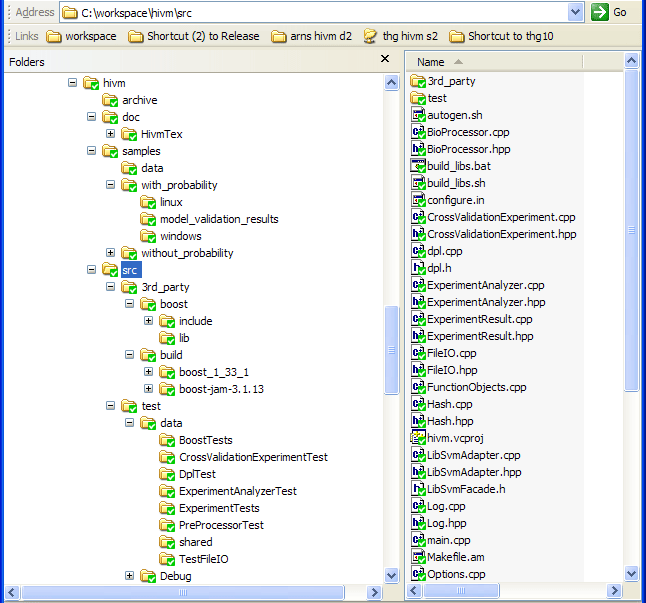
\includegraphics[height=1.00\textwidth]{images/descr_directories_files_hiv.png}
	\caption{Example of Directory and File Structure of hivm }
	\label{fig:descr_directories_files_hiv.png}
\end{figure}


\newpage

/root\newline
README.TXT - Usage and build guide.\newline
hivm.sln - Microsoft Visual Studio 7.1 solution file\newline

/src\newline
*.cpp, *.hpp, *.h, *.c - Source files\newline
autogen.sh - configuration script for *nix platform\newline
build\_libs.bat build\_libs.sh - script to build boost libraries for Windows or *nix\newline
Makefile.am - Main configuration file for automake\newline

/src/test\newline
*.cpp, *.hpp - Unit Test Source files\newline

/src/test/data/*\newline
*.tsv files - tab separated value files. Used by unit tests.\newline

/src/3rd\_party/boost/*\newline
Boost include and library files\newline

/src/3rd\_party/build/*\newline
Boost files needed to build binaries for a platform.\newline

/doc\newline
hivmSoftwaretodo-Schedule.xls - A list of software features, priority and estimated time to complete\newline
hivm-uml.vsd - MS Visio UML diagram\newline
libsvm.pdf - Libsvm documentation\newline

/doc/HivmTex\newline
Latex document file for Masters Thesis Culminating Experience Report\newline



/sample/data\newline
PI\_wild.seq - Wild type sequence file for HIV Protease enzyme\newline

PR\_2006-05-25\_v2.0.tsv - HIVDB Protease Inhibitor susceptibility file.\newline

cache.zip - Archive of all the cached local alignment values used in the default model selection and model validation scripts.  Unzip this to the same directory as the hivm executable to use them.\newline

/sample/[with\_probability|without\_probability]\newline
Identical directory structures, but scripts differ by use of the probability option for libsvm.\newline

/sample/with\_probability/\newline

README.TXT - Notes about scripts and results\newline

model\_validation\_results\_summary.xls - Summary of model validation vs model selection for best cost, gamma parameter pairs\newline

model\_selection\_results.zip - Archive of results from running model selection scripts \newline

\textbf{Files inside model\_selection\_results.zip}:\newline

APV-CrossValb\_t2* - drug, function (model selection) and threshold.\newline

*.log [APV-CrossValb\_t2.log] - Log files created during execution. \newline

*.cmdline.txt - All options used to run the experiment. Includes a command line script to recreate the experiment.\newline

*.results.csv - Contains the following aggregate information about cross-validation on the training dataset for each cost, gamma pair used in the grid search for optimal parameters:\newline

lg\_cost\newline
lg\_gamma\newline
P-error\newline
DOR (Diagnostic Odds Ratio)\newline
Sensitivity\newline 	
Specificity\newline 
PPV (Positive Predictive Value)\newline 
NPV (Negative Predictive Value)\newline 
Accuracy\newline 	
Error\_Rate\newline 
TPR minus FPR (True Positive Rate minus False Positive Rate)\newline
TP (True Positives)\newline 
FP (False Positives)\newline 
TN (True Negatives)\newline 
FN (False Negatives)\newline

*model\_selection\_ids.csv - Isolate name of every sequence used in training dataset for this experiment\newline

*roc\_data\_points.csv - The best data points from each false positive rate group are saved in this file.  This file is used to create the ROC curve\newline

*gnuplot\_script.plt - Gnuplot scripts generated during the model selection optimal parameter search.  These generate ROC curve images, labeled with different cost, gamma pairs.\newline

*roc\_curve.png - Image file of ROC curve. This is the output from the gnuplot script.\newline

/sample/with\_probability/model\_validation\_results/\newline

APV-modelValidation\_t2* - drug, function and threshold.\newline

*.prediction\_detailed\_results.csv - Contains the following information for every sequence in test dataset of model validation:\newline
Isolate	Predicted Susceptible (0 or 1)\newline
Actual Susceptibility (0 or 1)\newline
Probability\_of\_Prediction	 \newline
Lg\_Cost\newline
Lg\_Gamma\newline

*.log [APV-modelValidation\_t2.log] - Log files created during execution. \newline

*.cmdline.txt - All options used to run the experiment. Includes a command line script to recreate the experiment.\newline

*.results.csv - Contains the following aggregate information about cross-validation on the training dataset for each cost, gamma pair used in the grid search for optimal parameters:\newline

lg\_cost\newline
lg\_gamma\newline
P-error\newline
DOR (Diagnostic Odds Ratio)\newline
Sensitivity\newline 	
Specificity\newline 
PPV (Positive Predictive Value)\newline 
NPV (Negative Predictive Value)\newline 
Accuracy\newline 	
Error\_Rate\newline 
TPR minus FPR (True Positive Rate minus False Positive Rate)\newline
TP (True Positives)\newline 
FP (False Positives)\newline 
TN (True Negatives)\newline 
FN (False Negatives)\newline

*.trainset\_dataset\_ids.csv - Isolate name of every sequence used in training dataset for this experiment\newline

/sample/with\_probability/[linux or windows]\newline

The scripts to run model selection and model validation for each drug. Scripts are in Windows and Linux format.\newline

For example: NFV.sh and NFV.bat

[drug].sh - Script to run model-select on [drug] with thresholds 2 and threshold 10\newline

[drug]\_short.sh - Script with reduced grid search size for users wanting to run quick test of hivm\newline

model\_validate\_all.sh - Script to run model validation on all the drugs using cost, gamma parameters that created the best error rate in model selection for each drug\newline

hivm - The precompiled executable hivm file\newline

%----------------------------
%   CHAPTER : Results
%----------------------------
\chapter{Experimental Results and Analysis}
\label{cha:Experimental Results and Analysis}

\section{Model Selection Results}
\label{sec:Model Selection Results}

The model selection results were generated by scripts running simultaneously on several 3Ghz Pentium 4's over several days.  The model selection results for each drug are available in spreadsheet format in the following files:\newline
/hivm/samples/with\_probability/model\_selection\_results.zip\newline
/hivm/samples/without\_probability/model\_selection\_results.zip\newline

A detailed description of these files is available in the previous section entitled ``Description of Directories and Files''.

A detailed description of the model selection process can be found in the Libsvm Recommended Procedures for Model Selection, Implementation Challenges and Use Cases sections of this document.

\section{Model Validation Analysis}
\label{sec:Model Validation Analysis}

Analyzing our results via typical means has proved difficult.  We cannot compare our results directly to other programs that predict HIV drug resistance primarily because they only use nucleotide sequences for input data and hivm uses only amino acid sequences. In addition, hivm only predicts resistant or susceptible, while some other softwares predict for multiple classes of resistance. More detail on these issues can be found in the section entitled: Comparison to Similar Software. In addition, hivm's efficacy for clinical practice has been difficult to determine as we have not been able to get expert opinion on minimum acceptable performance levels. However, we can still make some observations about our model validation results.\newline

In general, specificity and sensitivity values below 60\% we consider poor, while we believe values above 90\% are  near the threshold of usefulness. Therefore, the preliminary results for our tests suggest that the following drugs may worth researching further: IDV, RTV, SQV, NFV\newline

In contrast, predicting  resistance for these drugs  using machine learning approach does not appear promising: ATV, APV, LPV \newline

Location of model-validation results for each drug:\newline
/hivm/samples/with\_probability/model\_validation\_results/APV-modelValidation\_t10\_results.csv\newline
/hivm/samples/without\_probability/model\_validation\_results/APV-modelValidation\_t10\_results.csv\newline

\textbf{OverFitting:}\newline

The difference in sensitivity and specificity between model selection and model validation tells us about overfitting. If the difference is 10 to 20\%, then the overfitting is  acceptably small. A greater difference suggests significant overfitting. This is important because if overfitting is small, we might justifiably use our entire dataset for training, and then use the cross-validation error of the optimal model as the final performance measure. With few exceptions, the difference in our experiments was below 10\% for both sensitivity and specificity, so this technique could help improve hivm's performance.

We used the lg cost, lg gamma pair with the lowest error-rate in model selection process to produce our model validation results. We have produced spreadsheets to more easily compare model selection vs model validation using these parameters. An example of the file is included in Figure 6.1.

Files detailing model validation results as compared against model selection results are available here:\newline
/hivm/samples/with\_probability/model\_validation\_results/model\_validation\_results\_summary.xls\newline
/hivm/samples/without\_probability/model\_validation\_results/model\_validation\_results\_summary.xls\newline

\newpage
\begin{figure}
	\centering
		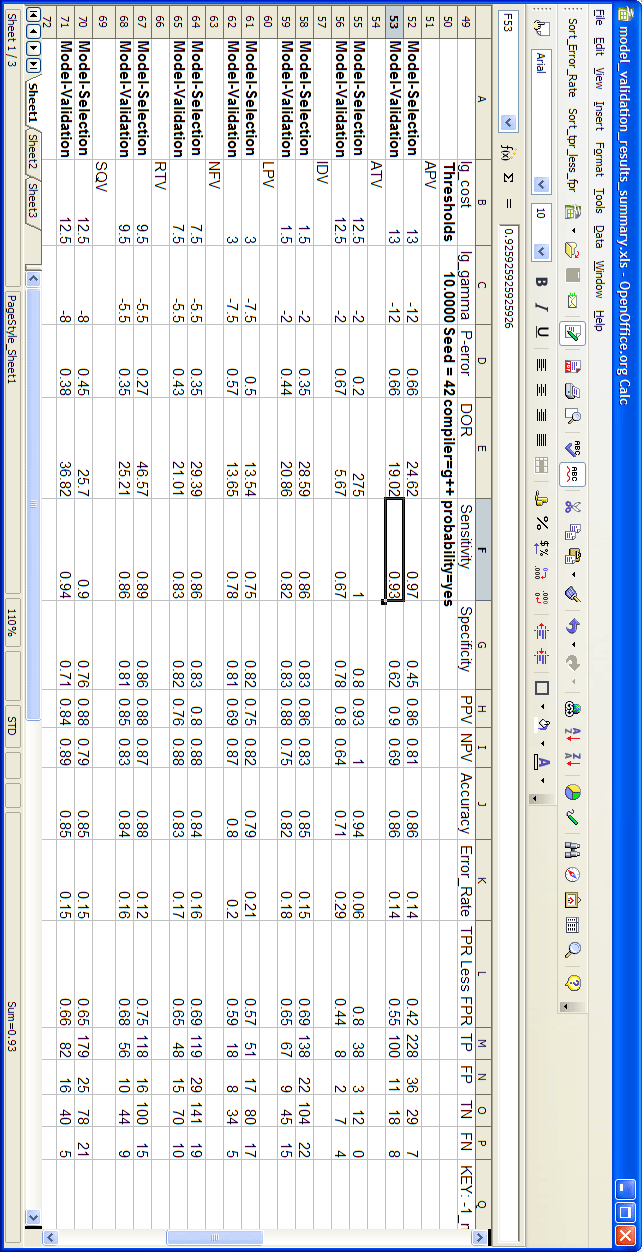
\includegraphics[width=1.00\textwidth, height=1.00\textheight]{images/model-validation-with-probability_summary_vertical.png}
	\caption{Summary of Best Model Selection vs Model Validation Results.}
	\label{fig:Model_Validation_summary}
\end{figure}
\newpage

\section{Probability vs Non-Probability Predictions}
\label{sec:Probability vs Non-Probability Predictions}
Libsvm supports prediction with or without an accompanying probability for the prediction. The two libsvm prediction functions sometimes produce different predictions for the same sequence. However, on the aggregate, this does not change the overall result. In addition, adding probability to the prediction gives a doctor more information about the quality of the prediction. For that reason, the model selection, model validation results with probability are preferred to those without probability.

Also, libsvm's prediction with probability function shows the variability among different compilers and math libraries. All results in hivm were produced on Linux Fedora Core 5, x86, 32bit with Gnu g++ 4.x

\section{Datasets}
\label{sec:Datasets}

The HIV Drug Resistance Database input datasets we use are updated periodically. The current (11/2004) datasets removed a substantial portion of previous data because the data much of the data was not high enough quality. Specifically, only one company's HIV resistance lab test, Virologic$^{TM}$, was included in the 11/2004 release.  We helped the HIV DB team discover an error that was made in the RT datasets. At the time of this writing, this dataset had not been corrected, so all results will only include the PI dataset.\cite{hivdb} Additionally, it was discovered that the HIVDB team was changing the 11/2004 datasets without notifying researchers. For that reason, we labeled my dataset with the date that we downloaded it: PR\_2006-05-25\_v2.0.tsv If a researcher downloads the supposed 11/2004 dataset again, it may have changed since 5/25/2006, and you will get different results from mine. Details of the errors may be found in the ``Issues with RT Dataset'' section of this document.

\section{Key to Results}
\label{sec:Key to Results}

We defined a positive result to mean that the given amino acid sequence was susceptible to the drug below the given threshold. Conversely, a negative result means that the sequence was resistant to the drug below a given threshold.\newline

TPR: True Positive Rate = Sensitivity\newline

Refers to the proportion of people with a disease who have a positive test result. In terms of hivm, it refers to the proportion of sequences which were susceptible to a drug below a given threshold and were correctly predicted to be susceptible below that threshold.\newline

FPR: False Positive Rate = 1 - Specificity\newline

Refers to the proportion of people without a disease who have a positive test result. In terms of hivm, it refers to the proportion of sequences which were resistant to a drug below a given threshold but were incorrectly predicted to be susceptible below that threshold.\newline

Specificity = True Negative Rate = TN/( FP + TN )\newline

Refers to the proportion of people without disease who have a negative test result. In terms of hivm, it refers to the proportion of sequences which were resistant to a drug below a given threshold and were correctly predicted to be resistant below that threshold.\newline

Error Rate: (FP+FN)/Total Experiments. Proportion of incorrect predictions.\newline

Positive Predictive Value: TP/(TP+FP)\newline

The probability that an individual with a positive test has a particular disease that the test is designed to detect. In hivm, the probability that an amino acid sequence with a positive prediction is actually susceptible to the drug below the given threshold.\newline

Negative Predictive Value: TN/(TN+FN)\newline

The probability that a subject with a negative test result actually does not have the disease. In hivm, the probability that a sequence with a negative prediction is actually resistant to the drug below the given threshold.\newline

Gamma: Lg gamma value used to train model for the test run.\newline

Cost:  Lg cost value used to train model for the test run.\newline

DOR: Diagnostic Odds Ratio - commonly used in medical applications\newline
DOR = (TP'/FN')/(FP'/TN')\newline
TP'=TP+0.5, FN'=FN+0.5, avoids the situation where DOR is undefined\newline

p-error: efficiency of SVM classifier with respect to a trivial classification rule.\newline
p-error = error rate/pmax\newline
pmax equals min(n1, n2)/(n1+n2)\newline

bestTprFprDifference: Greatest (TPR - FPR)\newline

A point that finds the maximum difference between the true positive rate and the false positive rate.\newline

TP = True  Positive = actual class 0, and predicted class 0 = sensitive hit\newline

FN = False Positive = actual class 0, but predicted class 1 = sensitive miss\newline

FP = False Positive = actual class 1, but predicted class 0 = resistant miss\newline

TN = True  Negative = actual class 1, but predicted class 1 = resistant hit\newline

AUC = Area Under ROC Curve\newline

\section{Thresholds}
\label{sec:Thresholds}
We chose threshold points of 2, 10 and also 2 and 10 simultaneously.

Though experts will want to control threshold more exactly, we used  ones that are widely regarded as 'low' and 'high' threshold for any HIV drug.\cite{seattletreatmentproj}

The combination of 2 and 10 was implemented, but proved fruitless. In order to implement it in a binary classification system, we had to remove all samples from the validation dataset that had thresholds greater than 2 or less than 10.  This manipulation of the validation dataset makes this test statistically invalid. The results from using the dual thresholds were overly optimistic. Furthermore, this approach could not be used in clinical use because we would have to remove all patients' samples that would fall between thresholds of 2 and 10 as hivm does not have a predictor for such samples. Of course, we do not know ahead of time which patients would fall into this category. We would not need hivm at all if we already knew that information.

In order to use two or more thresholds in a valid manner, hivm needs to be converted from binary classification to an n-ary classification implementation.

\section{Summary and Analysis of Results}
\label{sec:Summary and Analysis of Results}

We developed hivm for the purpose of evaluating an SVM (Support Vector Machine) based, machine learning application that could predict HIV drug resistance. We used a dataset of Virologic$^{TM}$ Protease Inhibitor phenotypic tests provided by the Stanford HIV Database team.\cite{hivdb} The drugs included in the dataset were: APV, ATV, IDV, LPV, NFV, RTV, and SQV. We evaluated hivm's performance by finding the optimal SVM model for the training data using 10-fold cross-validation and an optimal SVM parameter search. We then compared the optimal model's performance against the test dataset for thresholds 2 and 10 times greater than the normal drug dosage. These thresholds are widely regarded as the low and high cutoff points for HIV dosages.\cite{seattletreatmentproj}\newline

For the purposes of hivm, we defined a positive result to mean that the given amino acid sequence was susceptible to the drug below the given drug dosage threshold. Conversely, a negative result meant that the sequence was resistant to the drug below a given threshold. Thus sensitivity was a measure of hivm's ability to correctly detect sequences which were susceptible up to a given threshold of a particular drug. \newline

Evaluating the performance of hivm was a difficult task. The nature of our training data was incompatible with that used by all other contemporary softwares developed for this machine learning task. Additionally, the best available dataset was based on phenotypic tests instead of the preferable clinical trial data. Furthermore, we were unable to get expert opinion on the usefulness of hivm in clinical practice. This fact along with the phenotypic nature of our data,  made it very difficult to determine whether hivm exhibits clinically useful levels of performance.\newline

Despite this, we can say that hivm exhibited promise for certain drugs more than others. In particular, IDV, RTV, SQV, NFV may be of further research interest. They all exhibited simultaneous sensitivity and specificity levels greater than 80\% in some of our tests, and frequently had sensitivity or specificity levels greater than 90\%. In addition, they did not have particularly bad results in any of the tests of different thresholds. In contrast, ATV, APV, and LPV showed less promise. They did not typically reach the 90\% mark and occasionally exhibited very poor results. 

The different sample sizes likely impacted the results for each drug. RTV, SQV and NFV had the largest sample sizes of all the drugs, and they performed well.  In contrast, ATV and LPV had  dramatically smaller sample sizes than the other drugs. For this reason, they may yet be promising candidates if we can obtain more sample. Although APV frequently broke the 90th percentile in sensitivity, it also returned specificity scores below 60\% with a threshold of 10. However, it performed reasonably well for a threshold of 2.  APV had the most unusual results, and we are uncertain of a cause for this wide performance variability. 

Looking ahead, we hope to evaluate hivm with newly available clinical trial data. These results would give a better indication of hivm's ability as a new tool in clinical treatment for HIV positive patients. In addition, we hope the Stanford HIVDB team and others may experiment with hivm and shed more light on its potential clinical use. Through continued research, we hope that hivm may one day be used by experts as a tool for HIV treatment.

%----------------------------
%   CHAPTER : Conclusions
%----------------------------
\chapter{Conclusions}
\label{cha:Conclusions}

Overall, hivm showed mixed results for SVM based prediction of HIV drug resistance. We could not compare hivm directly against competing software due to incompatible input data and other issues; however, hivm did show promise for predicting phenotypic resistance of drugs: IDV, RTV, SQV, NFV. hivm may be more effective for drugs ATV and LPV if we could obtain more test samples using those drugs.

Looking ahead, we hope that the HIVDB team at Stanford and others may experiment with hivm, and shed more light on its potential clinical use. In addition, clinical trial data has recently become available. In order to evaluate the performance of hivm on this preferred data, a new preprocessor feature will need to be added to the application. This would give more insight into hivm's potential for clinical use.

In closing, one must remember that the results produced by hivm must still be evaluated by an expert before applying them in a clinical setting. hivm operates in a simplified model of HIV's interaction with the human body and an expert must account for those mitigating factors. However, the initial results from hivm do show promise for predicting resistance of certain HIV drugs. Through continued research, we hope that hivm may one day be used by experts as a tool for HIV treatment.%----------------------------
%   CHAPTER : FURTHER WORK
%----------------------------

\chapter{Future Work}
\label{cha:Future Work}

\section{Comparison to Similar Software}
\label{sec:Comparison to Similar Software}
In order to publish a paper about hivm, it needs to be compared against another software based method of drug resistance prediction. Unfortunately, the standard  input type for most software is nucleotide sequences, while the dataset for hivm was made from amino acid sequences. The function to transform nucleotide sequence to amino acid sequence is not one to one and therefore cannot be reversed. Requests to the Stanford HIVDB team for a nucleotide version of their susceptibility datasets have gone unanswered.

Prediction Software and Notes on Compatibility:\newline
Geno2Pheno: \cite{geno2pheno}

\textbf{Compatibility Issues:}\newline
Requires FASTA formatted nucleotide sequence of the pol gene for input.

What is the 'pol gene'.\newline
``pol: Codes for viral enzymes, the most important of which are reverse transcriptase, integrase, and protease which cleaves the proteins derived from gag and pol into functional proteins.'' \cite{polgene}\newline

According to the Geno2Pheno website, ``On submitting below an HIV-1 pol-gene DNA sequence you will obtain a sequence alignment to the reference strain HXB2, a list of mutations and different predictions of phenotypic resistance of the respective virus to 17 antiretroviral drugs.'' \cite{geno2pheno}

hivm predicts the protease enzyme separately from the reverse transcriptase using amino acid sequences for each enzyme.
It would be interesting to compare results for protease enzyme of running hivm on pol gene dna sequence vs running it on the protease amino acid sequence. We hypothesize that there would be less noise in the amino acid sequence data, and that it would produce better results to predict on the enzymes separately. Especially since the drugs in question target one enzyme or the other, but not both. The gene sequence always contains information on both enzymes at once.

However, in normal practice, a combination of drugs that target all the available enzymes is used simultaneously. Therefore, the pol gene method may have an advantage for predicting global resistance to different combinations of drugs.

\textbf{Stanford HIVDB HIValg} \cite{hivalg}

HIValg represents the best opportunity for comparison with hivm. \newline
According to the HIValg website, 
\begin{quotation}HIValg is designed for users interested in comparing the results of different algorithms or who are interested in comparing and evaluating existing and newly developed algorithms...HIValg also allows users to interpret sequences using any algorithm created using the Algorithm Specification Interface (ASI). Users can create their own algorithm and then upload it with their sequence.\cite{hivalg}\end{quotation}

HIValg has an option in their program to accept amino acid mutation lists in the format of the phenotypic datasets we have been using. However, here are the issues with it:
  
\begin{enumerate}
	\item It is a web form that is designed to be used manually. So, it would take hundreds of cut and pastes just to start the comparisons.
  
  \item The results are made for a human to look at, not for a machine to compile into statistics. Again, this requires a lot of labor to compile hundreds of sequence results. And rerunning the experiment would obviously be very tedious and time consuming.
  
  \item The program returns 5 classifications. (Which have been reduced to 3 by hivdb for comparison to some other algorithms.) hivm does binary classification. All of our statistics are based on binary classification using the confusion matrix. We estimate that it would take a lot of hours to recode hivm to handle 5 classes, and additionally we  could not use all the present stats that are based on the confusion matrix.
  
 	\item We would need to find out which fold resistance levels in the phenotypic sets are equal to the cutoffs in the hivdb 5 classification system. This is not published online, but we can ask them for guidance.  Also, it's interesting that the hivdb team does not publish results that compare their algorithm's results using their own phenotype datasets. They state that they only want to find out where various algorithms differ, and explore those sequences in more detail. It seems like they would have another way to measure their algorithm's performance.
  
  This also has an impact on comparing our results to hivdb's results. Unless we decide that the phenotype datasets are indeed the gold standard, we don't have a way to say which program produced the correct result whenever there is a discrepancy between the two programs.
    
 	\item hivdb team recently released a web service to accept nucleotide sequences into hivalg. However, they
  do not have a service for the mutation lists. If they create a web service for the mutation lists version of hivalg, then the first 2 problems could be eliminated. However, problems 3 and 4 still exist, and the web service requires new features to be added to hivm:\newline
  - web services capability must be added to hivm\newline
  - features to format input for web service\newline
  - feature to run statistics on the output of the web service\newline

\end{enumerate}

\section{Integrating Clinical Trial Data}
\label{sec:Integrating Clinical Trial Data}

hivdb team has recently released clinical trial results datasets. As previously stated, clinical trial data is much more useful than the datasets we used to generate our present results.  However, there are numerous problems we see with directly using this data with hivm.\cite{hivdb_clinical}\newline
  
  The Good:\newline
	Nucleotide datasets are provided, so it should be easier to compare hivm to other prediction software.\newline
	In GART and Havana trials, the measurements were taken at same periods  of time for all the patients.\newline
  
  Key Issue:\newline
	The patients all took different drug combinations. hivm handles results of one drug at a time that was grown in a test tube. We don't know how to prepare drug combination data for use with hivm.\newline
  
  \textbf{Other Differences:}
\begin{enumerate}
  \item Instead of the fold increases in the phenotypic datasets, they use:\newline
  a. CD4 counts\newline
  b. Viral Load
  \item Placebos were used
  \item In ACTG 320 and ACTG 364 trials, the measurements were taken over different periods of time for the patients. example, patient X was treated for 16 weeks only, but patient Y was treated for 40 weeks. Can their viral loads/CD4 counts be compared the same way? (Sections 3.1, 5.1, 5.2) \cite{hivdb_releasenotes}
\end{enumerate}
  
If the HivAlg team release a mutations list web service of HivAlg, it would become far easier to compare results with hivm. Presently, they have a  web service for using the hivdb expert system. \cite{hivdb_webservices}

\section{Source Forge}
\label{sec:Source Forge}
Placing hivm on Source Forge will hopefully spur many new users to try out hivm and provide valuable feedback for improving it's next release.

\section{Reverse Transcriptase}
\label{sec:Reverse Transcriptase}
HIVDB did not have a reliable dataset for HIV drugs that target the Reverse Transcriptase (RT) enzyme. When a reliable dataset becomes available, inclusion of RT drugs should be added.

\section{Support for Multiple Classifications}
\label{sec:Support for Multiple Classifications}
hivm currently supports only binary classification. One step toward comparing it to HIVAlg will be converting hivm to support greater than 2 classes. For example, low, medium and high resistance classes.

\section{More Detailed Data Analysis}
\label{sec:More Detailed Data Analysis}

Commenting on design of experiments, Cherkassky and Mulier note, ``Further it is important to make sure that past (training) data used for model estimation, and the future data used for predictions, come from the same (unknown) sampling distribution. If this is not the case, then (in most cases) predictive models estimated from the training data alone cannot be used for prediction with the future data.''\cite{learningfromdata} pg. 5\newline

Once we obtain some clinical trial data with patient responses, we need to analyze the data and make sure we are putting the correct prior knowledge into the SVM training model.  We already know that hivm should not necessarily predict patients' response well based on phenotypic/genotypic data. There could also be similar issues with data sets of the individual clinical trials. For instance, a trial from 1984 has a whole different clinical trial environment than a trial from 2004.  In the 1980's, the wild type virus was the primary strain being transmitted, and combination therapy was not widespread. In 2004, new patients often start with the wild type plus several resistant strains from the start. Furthermore, current patients are always treated with combination therapy.  Thus, we may be better served by using our knowledge of the the evolution of the HIV epidemic to partition the HIVDB data into sets that may represent different underlying sampling distributions. To be more explicit, the nature of drug resistance during these two example trial periods could be very different, and that will be represented in the data. Attempting to predict modern drug resistance from a 1980's data distribution may be impossible because the two datasets have different underlying distributions of the necessary features. Furthermore, mixing current datasets with the older datasets may significantly reduce hivm's performance. Proper organization and use of future patient response data could have a large impact on hivm's prediction rate for present day infections.

\section{Improved Speed}
\label{sec:Improved Speed}

In order to improve the computational performance of hivm, we plan to incorporate more advanced caching features into the application.  Many different results must be calculated in order to make a drug resistance prediction.  Many of these computation intensive partial results can be stored and automatically reused by hivm to speed up overall execution.


\section{Web Application or Web Service}
\label{sec:Web Application or Web Service}

In the event that hivm produces an accurate automatic predictor of the drug resistance in patients, an anonymous, secure hivm web application could be built for use in worldwide clinical practice.  First, a scientist obtains the appropriate amino acid  sequences of a patient's different HIV strains. This step must would require a blood sample being sent off to a 3rd party in order to return a digital copy of the patient's strains. Once this data is obtained, the scientist could put the amino acid sequences in a standard FASTA format plain text file, and upload this file anonymously through an web page front end to be processed by the hivm application on the back end. The scientist would be able to choose a global resistance level for the sequences: default, low, or high.  The web application would return a drug resistance profile for each amino acid sequence that was uploaded, detailing which drugs have been predicted to be effective for treating each strain of HIV, and how high the resistance level was set for each particular drug.\newline

 A 128-bit SSL (secure sockets layer)certificate would encrypt the data being transmitted. The web page could be run using a variety of web servers to interface with the compiled C++ hivm application on the server.   
 
\section{Alternative Local Alignment Algorithm}
\label{sec:Alternative Local Alignment Algorithm}
Different methods of sequence comparison could be used in the data preprocessing function of hivm that provides biological information into the SVM vectors. ``LA kernels suffer from the diagonal dominance problem, i.e. the fact that the kernel value decreases extremely fast with the similarity. SVMs are known not to perform well in such cases, and we therefore propose a modification of these kernels to overcome this issue, which involves taking their logarithm and ensuring that they remain positive definite after this operation by adding
a diagonal term.''\cite{vert}

 We would like to compare this method against our current local alignment algorithm to see how their performance compares.
\section{Structure Based Scoring}
\label{sec:Structure Based Scoring}
Create a BioProcessor based on predicted enzyme structure instead of enzyme sequence. Molecular docking shows a more detailed expectation for a drug's effectiveness on an HIV enzyme. We have access to very accurate experiment representations of the HIV enzymes' 3D structure. Many of the enzymes from patients only differ from the HIV wild type sequence by one or a few amino acid substitutions. While the overall field of computational molecular structure modeling can be extraordinarily computationally intensive, the problem of matching a single amino acid substitution against an experimentally known structure if a far simpler problem. A structure based scoring algorithm should be compared against the default Smith-Waterman algorithm to see which yields better performance.

\section{Exploring Variable Space and Storing Results}
\label{sec:Exploring Variable Space and Storing Results}
Given that testing n features creates an n x n matrix of results for a problem, it is not feasible to continue outputting hivm results into the present non-standard output files. We believe a database is needed if one is to really begin to study the impact of various features on hivm performance.  A set of queries on the database would be able to produce better representations of the results of using different combinations of features. \newline

There are more than ten variables selected during the different processing stages of hivm. Out of those ten, only gamma and cost had their possibility space searched.  It is possible that other parameters may be tuned to produce better results.

\section{Randomization within training data}
\label{sec:Randomization within training data}
We can expose a second seed to cause the training data in model selection to be randomized. If a model selection result seems like an outlier, this extra seed would be used to randomize the contents of the cross validation folds. Repeated running of the randomized folds would help show whether the result in question was an outlier or within normal bounds. 

\section{MS Visual Studio 8.0}
\label{sec:MS Visual Studio 8.0}
Running model selection under VS 8.0 compiled code leads to an apparent memory leak. hivm was primarily developed in VS 7.1 and g++ 4.1.1

\section{g++ and ROC Curve Creation}
\label{sec:g++ and ROC Curve Creation}
The g++ compiled code does not create a proper ROC curve dataset. It passes the unit tests for this code, but fails in normal execution. We cannot find a reason for this.

\section{MS Windows 7.1 and Virtual Memory}
\label{sec:MS Windows 7.1 and Virtual Memory}
When running a broad grid search of the largest datasets on VS 7.1 compiled code, the application exhausts the virtual memory of the system. This occurs on MS Windows systems with 2GB physical memory and 4GB virtual memory. When running identical code on the same hardware using a Virtual Machine of Fedora5 and using code compiled by g++ 4.1.1, the application always finishes the grid search.  This is true even when the Virtual Machine only gives 384MB of physical memory and 512MB of swap memory to the linux OS.

\section{Interface Directly into the HIVDB}
\label{sec:Interface Directly into the HIVDB}
Adding code to retrieve data over the Internet directly from the HIVDB using SQL would allow hivm have the latest dataset available. In addition, it would eliminate the problem of inconsistent formatting within the HIVDB tab delimited datasets. The database has a much more rigorous and well-defined design.

\section{Add output files to regression tests}
\label{sec:Add output files to regression tests}
The output files created by hivm are not part of the automated regression testing. This increases the likelihood that an error will be introduced into them. The Boost test library has a feature that could be implemented to test iostreams against reference files.\newline
http://www.boost.org/libs/test/doc/components/test\_tools/output\_test\_stream.html

\section{Add regression test logic for testing only public interfaces}
\label{sec:Add regression test logic for testing only public interfaces}
Add another layer of preprocessor definition logic to the unit tests so that public interfaces can easily be tested in isolation from implementation specific details.


\section{Standardizing HIVDB Input Data Format}
\label{sec:Standardizing HIVDB Input Data Format}
Working with HIVDB to choose a standard format for all their datasets, perhaps using an XML schema. As we look to incorporating the clinical trial data into the next version of hivm, we see a tremendous amount of work needed to preprocess the data. This wasted effort could be avoided by agreeing to a standard format for all their biological data. This should drastically reduce the time spent reformatting their data, and thus increase the amount of research performed as new data is released by HIVDB and other organizations.

%----------------------------
%   CHAPTER : ACKNOWLEDGEMENTS
%----------------------------

\chapter{Acknowledgements}
\label{cha:Acknowledgements}
First I would like to thank Ljubomir Buturovic for his patience, guidance and insight throughout the project. I would also like to thank my advisors, Dragutin Petkovic and Rahul Singh for their help. In addition, I would like to thank the various scholars from around the world that have corresponded with me during this project including, Jean-Philippe Vert (France), Chih-Jen Lin (Taiwan), and Robert Shafer and Soo-Yon Rhee (Palo Alto, CA).

\bibliographystyle{plain}

%----------------------------
%   BIBLIOGRAPHY
%----------------------------

\begin{thebibliography}{99}

\bibitem{jmolbiol81} J Mol Biol. 1981 Mar 25;147(1):195-7. Identification of common molecular subsequences. Smith TF, Waterman MS.

\bibitem{hivdb}  http://hivdb.stanford.edu

\bibitem{hivdbdatasets}  http://hivdb.stanford.edu/cgi-bin/GenoPhenoDS.cgi

\bibitem{nononsenseguide}  ``a no-nonsense guide to HIV drug resistance testing''. Horn and Richman, 
University of California San Diego

\bibitem{aidsorg} AIDS.ORG; http://www.aids.org/factSheets/125-Viral-Load-Tests.html

\bibitem{seattletreatmentproj}  An On-Line HIV Treatment Information Newsletter
From the Seattle Treatment Education Project, Volume 1, Issue 6, April 14, 2000, http://www.thebody.com/step/ezine\_apr00/genopheno.html

\bibitem{vert} H. Saigo, J.-P. Vert, T. Akutsu and N. Ueda, ``Protein homology detection using string alignment kernels'', Bioinformatics, vol.20, p.1682-1689, 2004.
http://cg.ensmp.fr/~vert/software/

\bibitem{projinfgenopheno}  http://www.projinf.org/fs/drugresist.html

\bibitem{shaferhivinsite}  Robert W. Shafer. Genotypic Testing for HIV-1 Drug Resistance.
HIV InSite Knowledge Base, 04/2004

\bibitem{learningfromdata}  Learning from Data, Cherkassky and Mulier, Ch. 9

\bibitem{libsvmtutorial}  
``A Tutorial on Support Vector Machines''
Pai-Hsuen Chen, Chih-Jen Lin, and Bernhard 

Department of Computer Science and Information Engineering
National Taiwan University
Taipei 106, Taiwan

\bibitem{libsvm} Chih-Chung Chang and Chih-Jen Lin, LIBSVM : a library for support vector machines, 2001. Software available at http://www.csie.ntu.edu.tw/~cjlin/libsvm


\bibitem{maxplanck}''Machine Learning with Positive Definite Kernels'', Bernhard Sch�olkopf, Max-Planck-Institut f�ur biologische Kybernetik, Empirical Inference Department Spemannstr. 38 72076 T�ubingen, Germany, bernhard.schoelkopf@tuebingen.mpg.de

\bibitem{svmintro} N. Cristianini and J. Shawe-Taylor. An Introduction to Support Vector Machines and other kernel-based learning methods. Cambridge University Press, 2000.

\bibitem{biowulf} Nello Cristianini, BIOwulf Technologies, nello@support-vector.net, 
http://www.support-vector.net/tutorial.html, http://www.support-vector.net/icml-tutorial.pdf

\bibitem{wolfram}  Wolfram Research: MathWorld, http://mathworld.wolfram.com/HilbertSpace.html

\bibitem{mitlicense} http://www.opensource.org/licenses/mit-license.php

\bibitem{libsvmpraticalguide}  A Practical Guide to Support Vector Classification
Chih-Wei Hsu, Chih-Chung Chang, and Chih-Jen Lin
Department of Computer Science and
Information Engineering
National Taiwan University
Taipei 106, Taiwan (cjlin@csie.ntu.edu.tw)

\bibitem{roc}http://gim.unmc.edu/dxtests/roc3.htm, Thomas G. Tape, MD, University of Nebraska Medical Center

\bibitem{vapniknature} Vapnik, V. (1995). The Nature of Statistical Learning Theory. New York, NY:
Springer-Verlag.

\bibitem{straingapplied} Straing, Gl, Introduction to Applied Mathematics, Wellesle, MA: Wellesley-Cambridge Press, 1986.

\bibitem{neuralcomputation} Keerthi, S. S. and C.-J. Lin (2003). Asymptotic behaviors of support vector machines
with Gaussian kernel. Neural Computation 15 (7), 1667�1689.

\bibitem{linsigmoidkernels} Lin, H.-T. and C.-J. Lin (2003). A study on sigmoid kernels for SVM and the training
of non-PSD kernels by SMO-type methods. Technical report, Department
of Computer Science and Information Engineering, National Taiwan University.
Available at http://www.csie.ntu.edu.tw/~cjlin/papers/tanh.pdf.

\bibitem{leakdetector} http://www.codeproject.com/tools/visualleakdetector.asp

\bibitem{valgrind}http://valgrind.org/

\bibitem{libsvm_acknowledgments}http://www.csie.ntu.edu.tw/\~cjlin/libsvm/acknowledgements

\bibitem{geno2pheno}http://www.geno2pheno.org/cgi-bin/geno2pheno.pl

\bibitem{polgene} http://en.wikipedia.org/wiki/HIV\_structure\_and\_genome

\bibitem{hivalg}http://hivdb.stanford.edu/pages/algs/HIValg.html

\bibitem{hivdb_clinical}http://hivdb.stanford.edu/pages/clinicalStudyData/ACTG320.html

\bibitem{hivdb_releasenotes}http://hivdb.stanford.edu/pages/asi/releaseNotes/

\bibitem{hivdb_webservices}http://hivdb.stanford.edu/pages/webservices/

\bibitem{empiricalmap} W. Noble,
``Support Vector Machine Applications in Molecular Biology.'' in
B. Schoelkopf, K. Tsuda and J.-P. Vert (eds.), Kernel Methods in
Computational Biology. MIT Press, 2004, pp. 71-92.

\bibitem{larman}``Applying UML and Patterns: An Introduction to Object-Oriented Analysis and Design and the Unified Process'', 2nd Edition. by Craig Larman

\bibitem{baker}Stuart G. Baker, ''The Central Role of Receiver Operating Characteristic (ROC) Curves in Evaluating Tests for the Early Detection of Cancer'', Journal of the National Cancer Institute, Vol. 95, No. 7, April 2, 2003

\bibitem{gnuplot}http://www.gnuplot.info/

\bibitem{crossvalidation}http://www.cs.cmu.edu/~schneide/tut5/node42.html

\bibitem{rocdef}http://www.cs.ucl.ac.uk/staff/W.Langdon/roc/

\end{thebibliography}

\end{document}
